
%% FAZIT %% 
\clearpage
\appendix
\addcontentsline{toc}{chapter}{Appendix} 
\newcommand{\nocontentsline}[3]{}
\newcommand{\tocless}[2]{\bgroup\let\addcontentsline=\nocontentsline#1{#2}\egroup}

\tocless\chapter{Details of Survey 1}
\begin{center}
\begin{figure}[H]
	\centering
	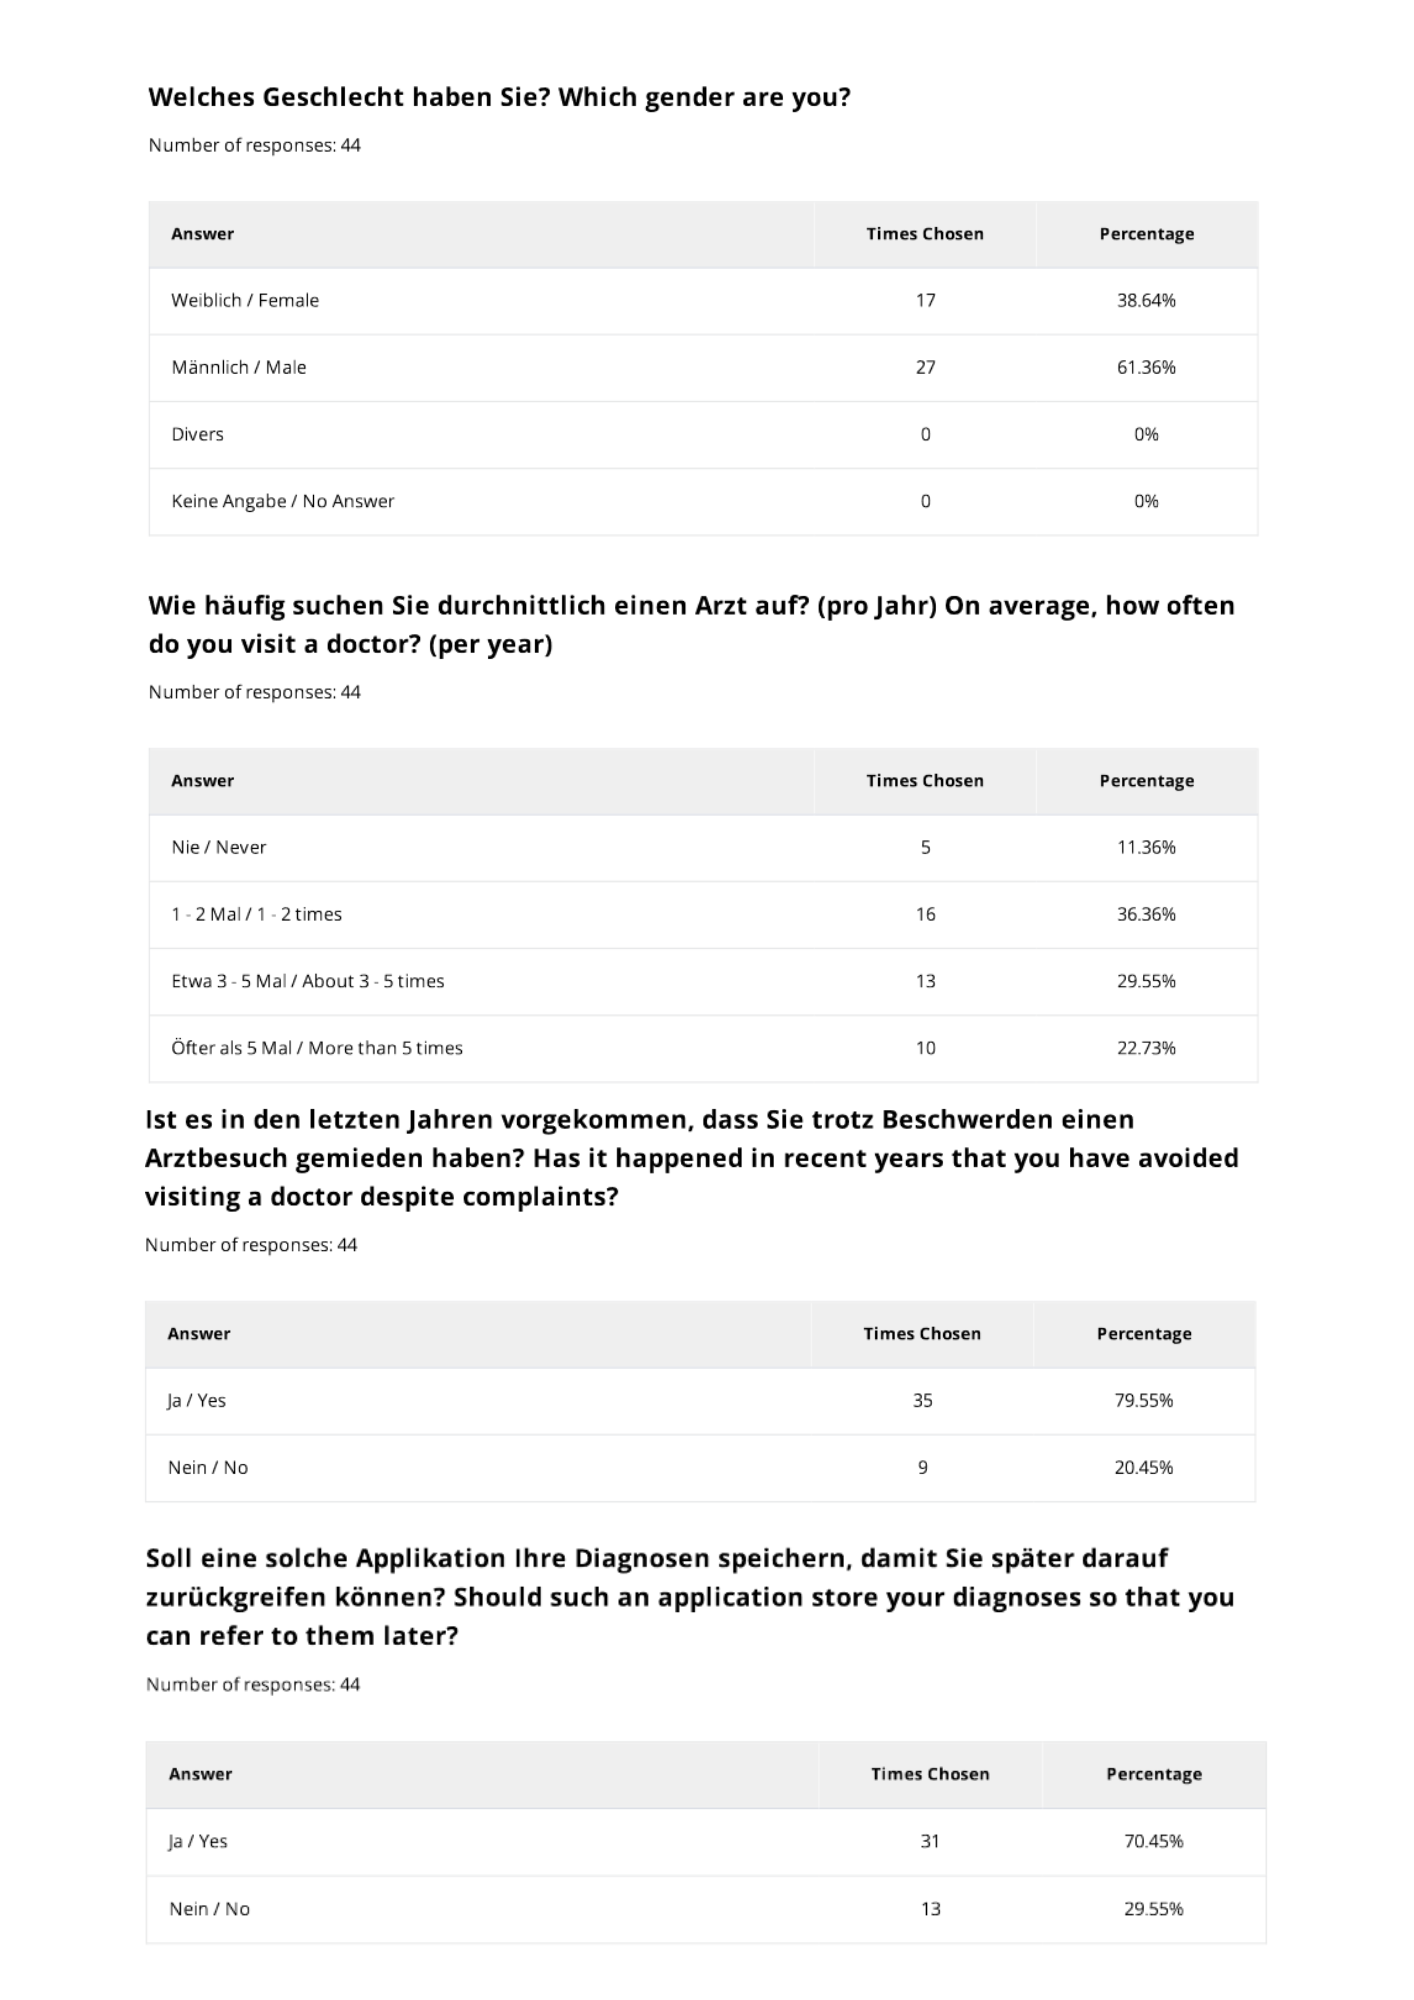
\includegraphics[scale=0.6]{umfrage11.png}
			\caption{Survey 1, Questions 1 - 4}
\end{figure}
\begin{figure}[H]
	\centering
	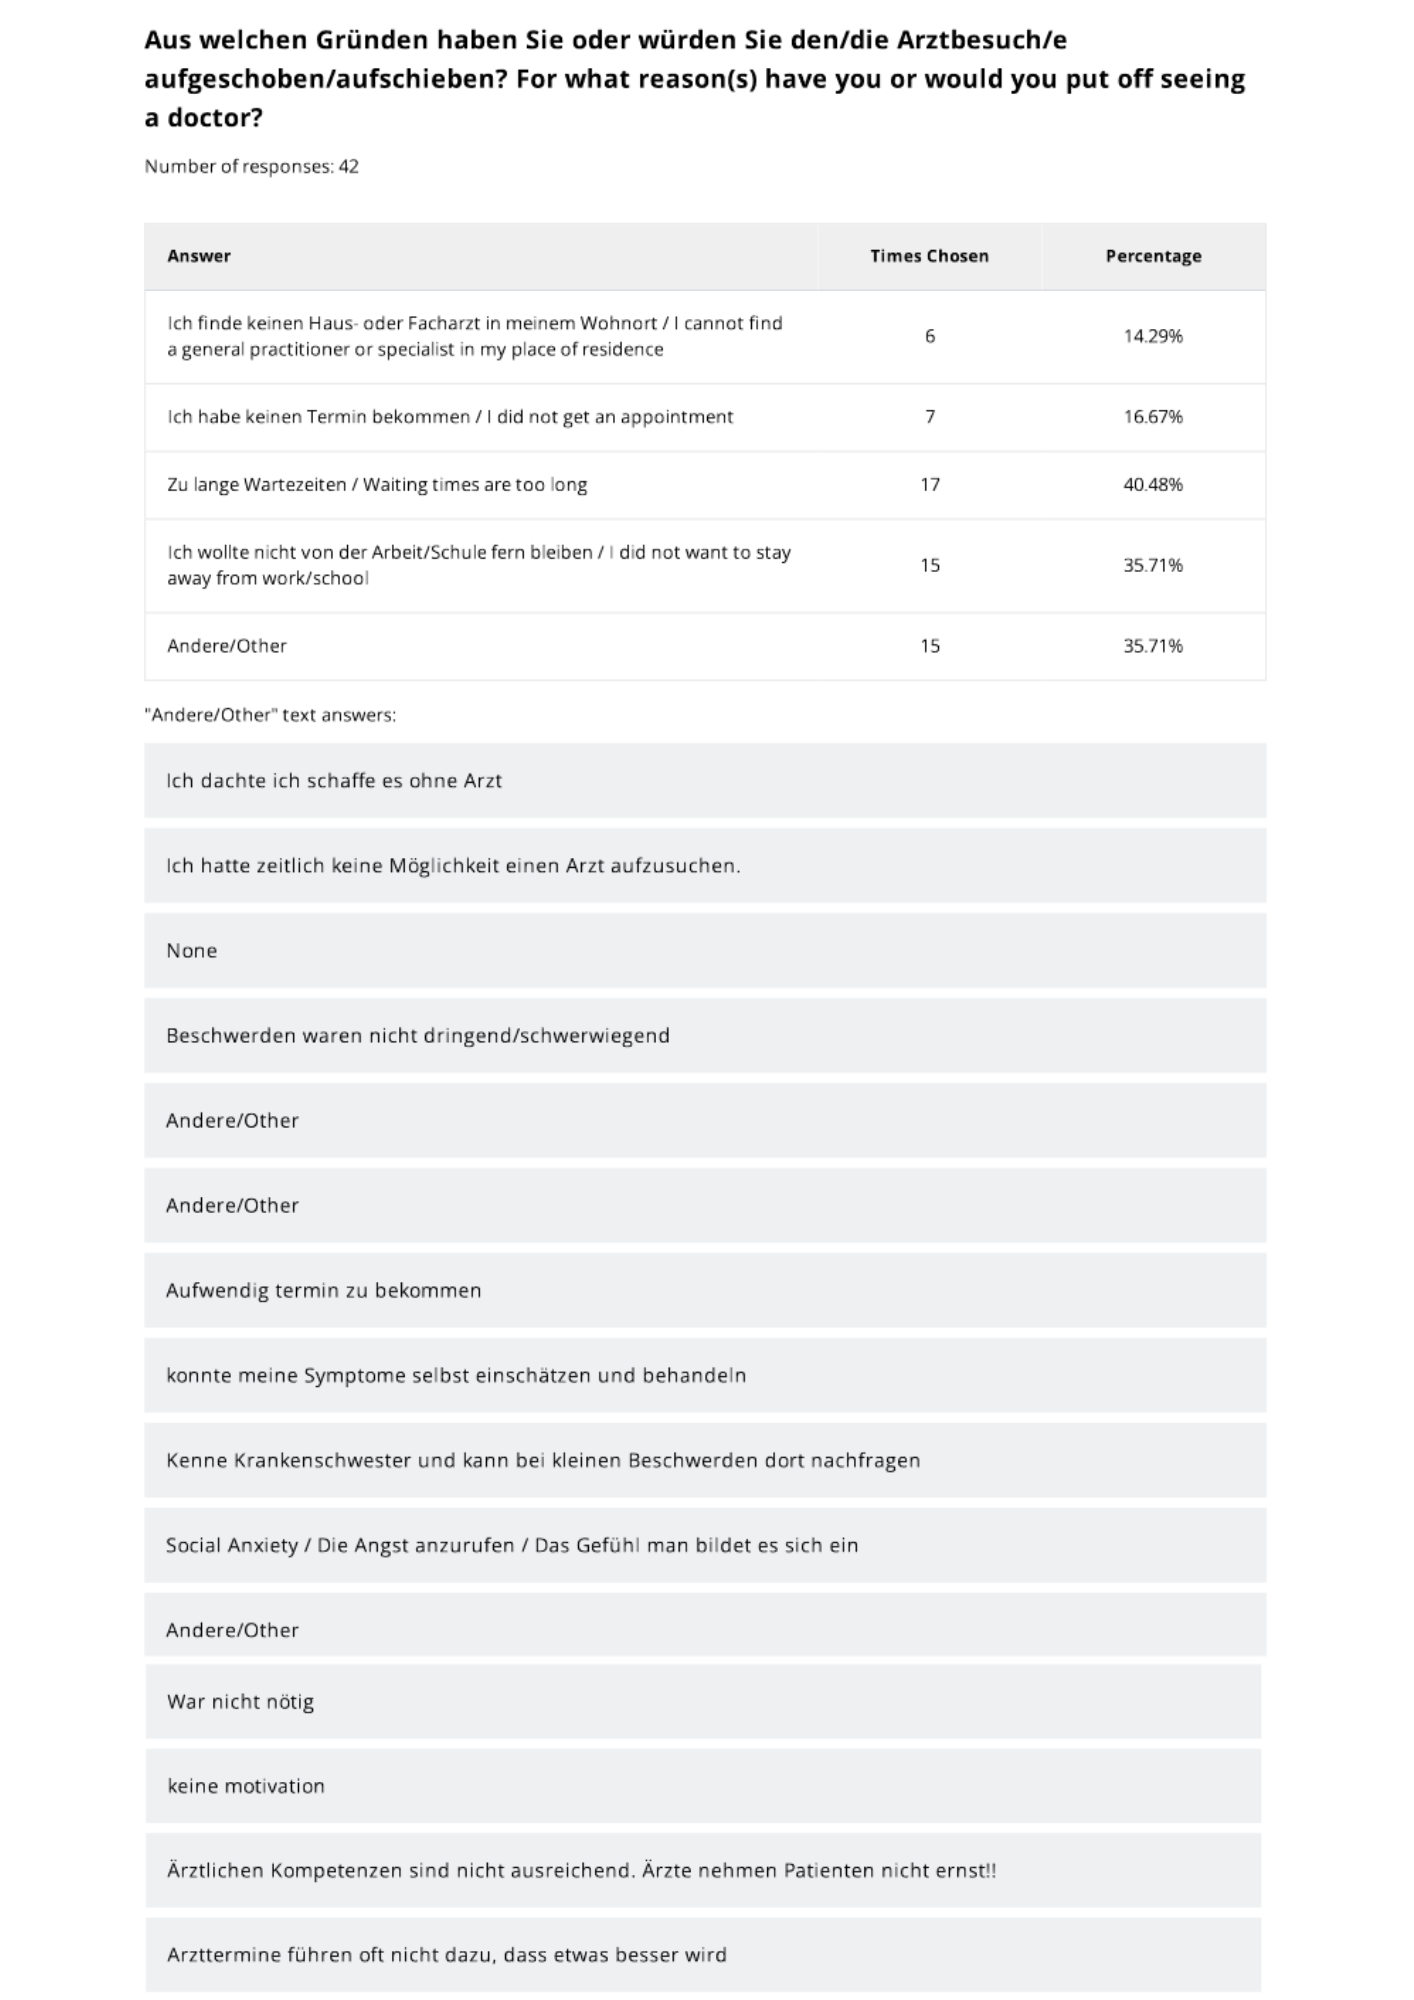
\includegraphics[scale=0.7]{umfrage12.png}
		\caption{Survey 1, Question 5}
\end{figure}
\begin{figure}[H]
	\centering
	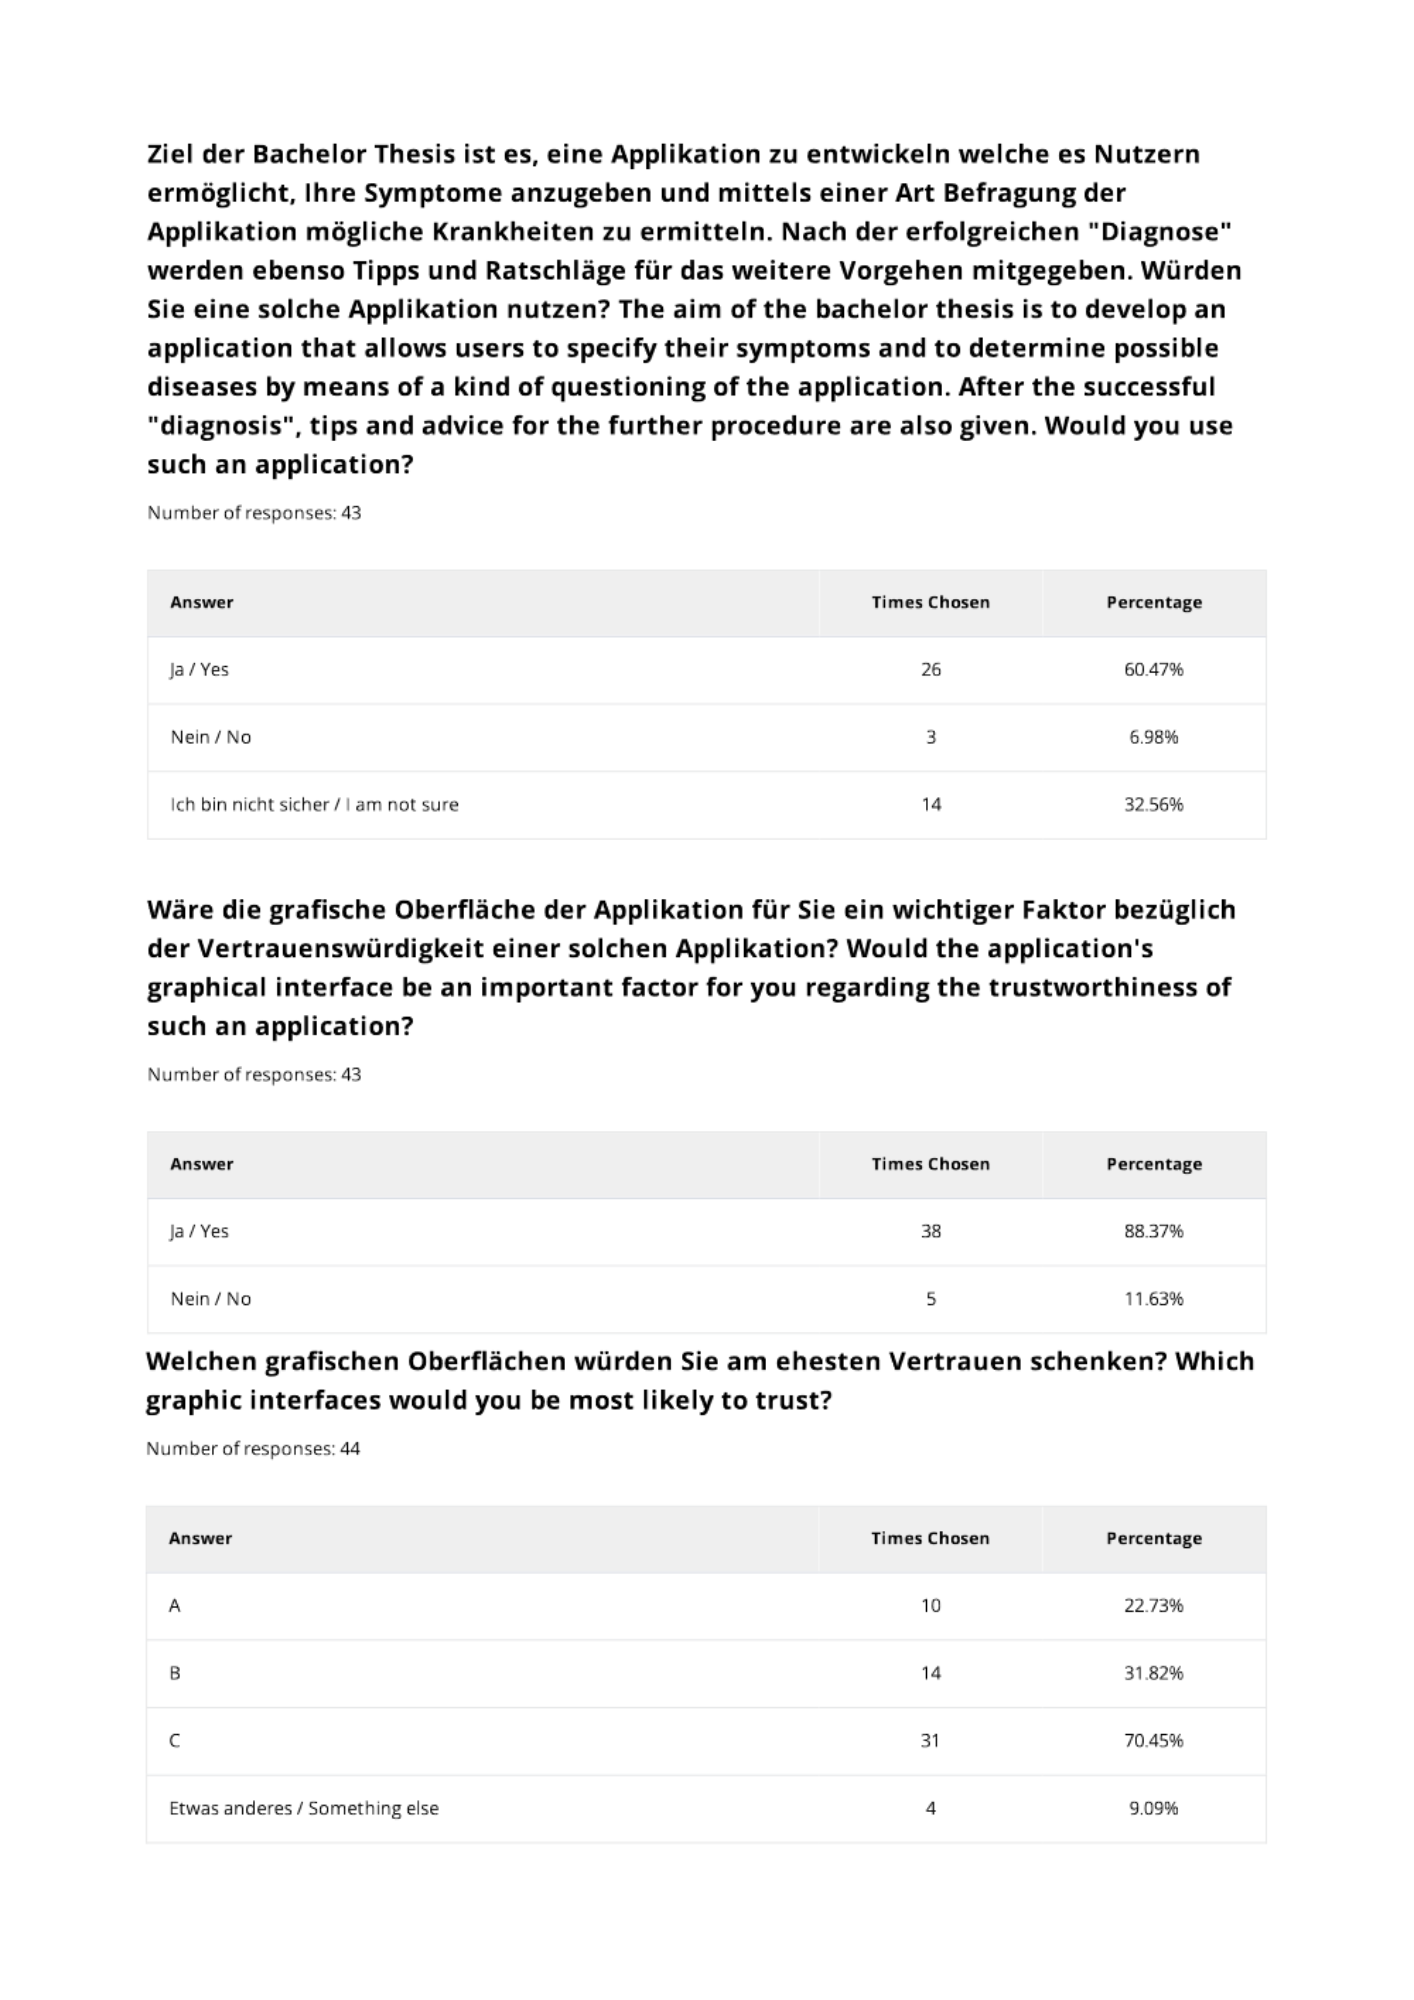
\includegraphics[scale=0.7]{umfrage13.png}
	\caption{Survey 1, Questions 6 - 8}
\end{figure}
\end{center}
\pagebreak


\tocless\chapter{Code Snippet of Widget Tree}
\begin{lstlisting}[language=Python, caption={Code Snipped of Widget Tree}]
Widget build ( BuildContext context ) {
	 return Scaffold(
		 appBar: AppBar (
		 	title : const Text('Example of the build method') ,
	 	 ),
		 body : const Center(
		 	child : Text('Hello Reader') ,
		 ),
	 );
}
\end{lstlisting}
\pagebreak


\tocless\chapter{Overview of the Requirements}
\tocless\section{Optional Requirements}
\begin{table}[H]
	\begin{center}
		\scriptsize
		\def\arraystretch{1.5}%
		\begin{tabular}{ c|l }
			\hline
			\textbf{ID} & \textbf{Description}  \\
			\hline
			OR1 & The application should make it possible to save and download a diagnosis in PDF format  \\
			\hline
			OR2 & The application should make it possible for a user to save tips on a favorites list  \\
			\hline	
		\end{tabular}
		\normalsize
	\end{center}
	\caption{Optional Requirements}
\end{table}
\tocless\section{Function Requirements}
\begin{table}[H]
	\begin{center}
		\scriptsize
		\def\arraystretch{1.5}%
		\begin{tabular}{ c|l}
			\hline
			\textbf{ID} & \textbf{Description}  \\
			\hline
			FR1 & The application must allow the user to switch between the diagnostics and the advices view  \\
			\hline
			FR2 & The application must offer the user the option of being able to verify themselves as a doctor  \\
			\hline
			FR3 & The application must offer a doctor the opportunity to log in  \\
			\hline
			FR4 & The application must offer a doctor the opportunity to add a new record in the database  \\
			\hline
			FR5 & The application must offer a doctor the possibility of editing data records in the database  \\
			\hline
			FR6 & The application must allow a user to start a new diagnosis  \\
			\hline
			FR7 & The application must enable a user to save a diagnosis  \\
			\hline	
			FR8 & The application must enable a user to view his saved diagnoses again  \\
			\hline
			FR9& The application must allow a user to abort his diagnostic procedure at any time \\
			\hline
			FR10 & The application must allow a user to delete saved diagnoses  \\
			\hline
			FR11 & The application must allow a doctor to abort adding or editing data at any time\\
			\hline
		\end{tabular}
		\normalsize
	\end{center}
	\caption{Functional Requirements}
\end{table}

\tocless\section{Non-functional Requirements}
\begin{table}[H]
	\begin{center}
		\scriptsize
		\def\arraystretch{1.5}%
		\begin{tabular}{ c|l }
			\hline
			\textbf{ID} & \textbf{Description}  \\
			\hline
			NFR1 & The application must make correct diagnoses  \\
			\hline
			NFR2 & The application must be usable for patients without registration  \\
			\hline
			NFR3 & The application should have a graphical interface that can be used intuitively  \\
			\hline	
		\end{tabular}
		\normalsize
	\end{center}
	\caption{Non-Functional Requirements}
\end{table}
\pagebreak



\tocless\chapter{Use Cases}
\begin{table}[H]
	\begin{center}\scriptsize
		\def\arraystretch{2}%
		\begin{tabular}{ c|c } 
			\hline
			Name & Get Diagnosis \textbf{[FR6]}\\
			\hline	
			Description & The user wants to get a diagnosis, based on their symptoms \\ 
			\hline
			Result & The user receives a diagnosis \\ 
			\hline
			Actors & User, Doctor \\ 
			\hline
			Trigger & The user clicks on the new diagnosis button \\ 
			\hline
			Preconditions & None \\ 
			\hline
			Steps & \parbox{9cm}{\vspace{.5\baselineskip}
				1. The user clicks on the new diagnosis button\\
				2. The system displays the view to enter and specify symptoms\\
				3. The user selects his symptoms and specifies them\\
				4. The user indicates that he is finished\\
				5. Diagnosis: the system determines possible diseases and presents them to the user and the use case ends}\\
			\hline
			Alternate flow & \parbox{9cm}{
				AF1a. The user wants to cancel the diagnosis and presses the stop button \textbf{[FR10]}\\
				AF1b. The system returns to the main page of the application\\\\
				AF2a. The user wants to save the diagnosis \textbf{[FR7]}\\
				AF2b. The user presses the save button\\
				Af2c. The system saves the diagnosis
			}\\ 
			\hline
		\end{tabular}\normalsize
	\end{center}
	\caption{Use case get diagnosis}
\end{table}
\begin{table}[H]
	\begin{center}\scriptsize
		\def\arraystretch{2}%
		\begin{tabular}{ c|c } 
			\hline
			Name & Review received diagnosis \textbf{[FR8]}\\
			\hline	
			Description & The user wants to review a diagnosis one more time \\ 
			\hline
			Result & The system shows the selected diagnosis to the user\\ 
			\hline
			Actors & User, Doctor \\ 
			\hline
			Trigger & Click on the diagnosis \\ 
			\hline
			Preconditions & The user has previously saved the diagnosis \\ 
			\hline
			Steps & \parbox{9cm}{\vspace{.5\baselineskip}1. The user selects the diagnosis from a list of previously stored diagnoses\\2. The system shows the selected diagnosis to the user \\ 3. When finished the user clicks on the back button}\\
			\hline
			Alternate flow & \parbox{9cm}{\vspace{.5\baselineskip}
				AF1a. The user wants to delete the diagnosis \textbf{[FR12]}\\
				AF1b. The user clicks on the delete button\\
				AF1c. The system deletes the diagnosis\\\\
				AF2a. The user wants to download the diagnosis as PDF\\
				AF2b. The user presses the download button}\\
			\hline
		\end{tabular}\normalsize
	\end{center}
	\caption{Use case review received diagnoses}
\end{table}
\begin{table}[H]
	\begin{center}\scriptsize
		\def\arraystretch{2}%
		\begin{tabular}{ c|c } 
			\hline
			Name & Get Tips and Tricks for Symptoms and Diseases \textbf{[FR13]}\\
			\hline	
			Description & The user wants to see tips and tricks regarading their symptoms \\ 
			\hline
			Result & The system shows the tip-view to the user\\ 
			\hline
			Actors & User, Doctor \\ 
			\hline
			Trigger & Click on the tip tab\\ 
			\hline
			Preconditions & None \\ 
			\hline
			Steps & \parbox{9cm}{\vspace{.5\baselineskip}
				1. The user selects the tip tab on the bottom navigation bar\\
				2. The system displays the tip-dashboard\\
				3. The user clicks on a tip to see the whole tip-description\\
				4. The system displays the tip-detail-page and the use case ends}\\
			\hline
			Alternate flow & \parbox{9cm}{\vspace{.5\baselineskip} 
				AF1a. The user wants to add a tip to his favorites \textbf{[OR2]}\\
				AF1b. The user clicks on the favorite icon of the tip\\
				AF1c. The system saves the tip to the users favorites }\\
			\hline
		\end{tabular}\normalsize
	\end{center}
	\caption{Use case get tups and tricks for sympstoms and diseases}
\end{table}
\begin{table}[H]
	\begin{center}\scriptsize
		\begin{tabular}{ c|c } 
			\hline	
			Name & Login \textbf{[FR3]}\\ 
			\hline	
			Description & The user, a doctor, wants to log into the application \\ 
			\hline
			Goal & The doctor successfully logged into the system \\ 
			\hline
			Actors & Doctor \\ 
			\hline
			Trigger & Click on the login button \\ 
			\hline
			Preconditions & User is verified as a doctor \textbf{[FR3]} \\ 
			\hline
			Steps & \parbox{9cm}{\vspace{.5\baselineskip}
				1. The doctor clicks on the login button\\
				2. The systems shows the login form\\
				3. The doctor enters his personal details and presses the okay button\\
				4. The system checks for the credentials in the database\\
				5. The system displays the Add screen and the use case ends\\}\\
			\hline
			Alternate flow & \parbox{9cm}{\vspace{.5\baselineskip}
				AF1a. The system could not find the given credentials in the database\\
				AF1b. The user entered wrong credentials\\
				AF1c. The system displays an error message\\
				AF1d. The user retries\\\\
				AF2a. The user is not verfied as doctor yet \textbf{[FR3]}\\
				AF2b. The doctor enters his personal details and presses the okay button\\
				AF2c. The system starts the verification method\\
				AF2d. The doctor is verified as doctor\\
				AF2e. The system displays the Add screen and the use case ends\\}\\ 
			\hline
			Alternate flow (failure) & \parbox{9cm}{\vspace{.5\baselineskip}
				AFF1a. The user is no doctor\\
				AFF1b. The user is not able to verify himself as doctor\\
				AFF1c. The system shows an error}\\
			\hline
		\end{tabular}
	\end{center}\normalsize
	\caption{Use case login}
\end{table}
\begin{table}[H]
	\begin{center}\scriptsize
		\begin{tabular}{ c|c } 
			\hline	
			Name & Add data to the databas  \textbf{[FR4]} \\
			\hline
			Description & The actor wants to add new data to the database \\ 
			\hline
			Goal & The data is added to the database \\ 
			\hline
			Actors & Doctor, Developer \\ 
			\hline
			Trigger & Click on the addData button \\ 
			\hline
			Preconditions & Actor is logged in \\ 
			\hline
			Steps & \parbox{9cm}{\vspace{.5\baselineskip}
				1. The actor clicks on the addData button\\
				2. The system shows the add form\\
				3. The actor enters the required data and presses the ok button\\
				4. The system adds the disease, symptom, cause or tip to the database\\ } \\
			\hline
			Alternate flow & \parbox{9cm}{\vspace{.5\baselineskip}
				AF1a. The actor missed to enter data\\
				AF1b. The system displays an error message\\
				AF1c. The actor retries\\\\
				AF2a. The actor wants to cancel the process \textbf{[FR12]}\\
				AF2b. The actor clicks on the cancel button\\
				AF2c. The system closes the add form}\\ 
			\hline
		\end{tabular}
	\end{center}\normalsize
	\caption{Use case add data}
\end{table}
\begin{table}[H]
	\begin{center}\scriptsize
		\begin{tabular}{ c|c }
			\hline
			Name & Edit Data \textbf{[FR5]} \\ 
			\hline	
			Description & The actor wants to edit old data \\ 
			\hline
			Goal & The edited data is uploaded to the database \\ 
			\hline
			Actors & Doctor, Developer \\ 
			\hline
			Trigger & Click on the edit button \\ 
			\hline
			Preconditions & Actor is logged in \\ 
			\hline
			Steps & \parbox{9cm}{\vspace{.5\baselineskip}
				1. The actor clicks on the edit button on the data he wants to edit\\
				2. The system shows the edit form\\
				3. The actor edits the data and presses the okay button\\
				4. The system updates the data and the use case ends
			}\\
			\hline
			Alternate flow & \parbox{9cm}{\vspace{.5\baselineskip}
				AF1a. The actor wants to cancel the process \textbf{[FR12]}\\
				AF1b. The actor clicks on the cancel button\\
				AF1c. The system closes the edit form}\\ \\ 
			\hline
		\end{tabular}
	\end{center}\normalsize
	\caption{Use case edit data}
\end{table}

\newpage
\scriptsize
\tocless\chapter{Response of the APIs}

\tocless\section{Response of the NHS API (abbreviated)}
A full response can be viewed by scanning the QR code shown below. 
\begin{lstlisting}[caption={Abbreviated Response of NHS API}]
	{
		"@context":"http://schema.org",
		"@type":"MedicalWebPage",
		"name":"Acne",
		"copyrightHolder":{...},
		"license":"https://developer.api.nhs.uk/terms",
		"author":{...},
		"about":{...},
		"description":"...",
		"url":"https://api.nhs.uk/conditions/acne/",
		"genre":[...],
		"keywords":[...],
		"lastReviewed":[...],
		"breadcrumb":{...},
		"dateModified":"2022-05-30T14:30:18+00:00",
		"hasPart":[...],
		"relatedLink":[...],
		"contentSubTypes":[...],
		"mainEntityOfPage":[...],
		"alternativeHeadline":"Overview"
	}
\end{lstlisting}
\begin{figure}[H]
	\centering
	
\includegraphics[scale=0.25]{nhsresponsegithub.png}
	\caption{QR-Code NHS API Response, GitHub}
\end{figure}
The QR code redirects to a GitHub repository created for this bachelor thesis. If the code does not work anymore due to an error, you can simply go to the following address in your web browser:
\begin{center}
	\url{https://github.com/petzolan/disease_detection/blob/main/NHS_response.json}
\end{center}
\pagebreak
\tocless\section{Response of the ApiMedic API}
\textit{All diseases (abbreviated):} 

\begin{lstlisting}[basicstyle=\tiny, caption={Abbreviated Reponse of all Diseases ApiMedic API}]
[
	{
		"ID":130,
		"Name":"Abdominal hernia"
	},
	{
		"ID":170,
		"Name":"Abortion"
	},
	{
		"ID":456,
		"Name":"Abscess of the tonsils"
	},
	{
		"ID":577,
		"Name":"Absence seizure"
	},
	{
		"ID":584,
		"Name":"Accident injury"
	},
...
\end{lstlisting}

\vspace{1cm}
\textit{Disease with the ID 105:} 
\begin{lstlisting}[basicstyle=\tiny, caption={Response ApiMedic API (issue ID 105)}]
{
	"Description": "Measles is caused by a virus and is very contagious. Measles can be very unpleasant and can lead sometimes to serious complications. Anyone can get measles if he has not been vaccinated. People who did not have measles before can also get it if they come in contact with an infected person. However, the condition is most common in young children. The infection disappears usually in around 7 to 10 days.",
	
	"DescriptionShort": "Measles, also known as morbilli, is a viral infection that commonly affects children and causes a skin rash, fever, and swelling of the lymph nodes. It is very contagious and there is a vaccine for it.",
	
	"MedicalCondition": "The infection begins with flu-like symptoms (runny nose, fever, cough) and subsequently develops into a fever and a rash with large spots that spread from the head downward. The lymph nodes are also swollen enough to be felt. Because the measles weakens the immune system, other dangerous secondary infections of the lung or brain can develop. The measles can remain undetected for several years after the initial attack and attack the brain, which can lead to death.",
	
	"Name": "Measles",
	
	"PossibleSymptoms": "Burning eyes,Burning in the throat,Cough,Eye redness,Fever,Itching eyes,Pain in the limbs,Runny nose,Skin rash,Sore throat,Swollen glands in the armpit,Swollen glands in the groin,Swollen glands in the neck,Tiredness,Oversensitivity to light,Facial swelling,Flaking skin",
	"ProfName": "Morbilli",
	
	"Synonyms": "Red measles",
	
	"TreatmentDescription": "To prevent measles, an effort to vaccinate the entire population is being undertaken to protect from the consequences of the infection. Two shots are required, the first one at 12 months of age and the second at 15-24 months. The shot is combined with other vaccines for measles, mumps, and rubella (MMR). If an infection with measles occurs, the infected child should not be allowed contact with other children for 5 days after the outbreak of the rash to prevent the infection from spreading.  People who have come in contact with the infected child (classmates, for example) and who have not had measles or been vaccinated against them should stay at home for 14 days for the same reason. There is no treatment for measles. The only protection against measles is the vaccination or a previous measles infection."	
}
\end{lstlisting}



\pagebreak
\tocless\chapter{Jupyter Notebook (QR-Code)}
\begin{figure}[H]
	\centering
	
\includegraphics[scale=0.25]{juypternotebookgithub.png}
	\caption{QR-Code JupyterNotebook, GitHub}
\end{figure}
The QR code redirects to a GitHub repository created for this bachelor thesis. If the code does not work anymore due to an error, you can simply go to the following address in your web browser:
\begin{center}
	\url{https://github.com/petzolan/disease_detection/tree/main/%5BjuypterNotebook%5D}
\end{center}



\tocless\chapter{Details of Survey 2}
\begin{center}
	\begin{figure}[H]
		\centering
		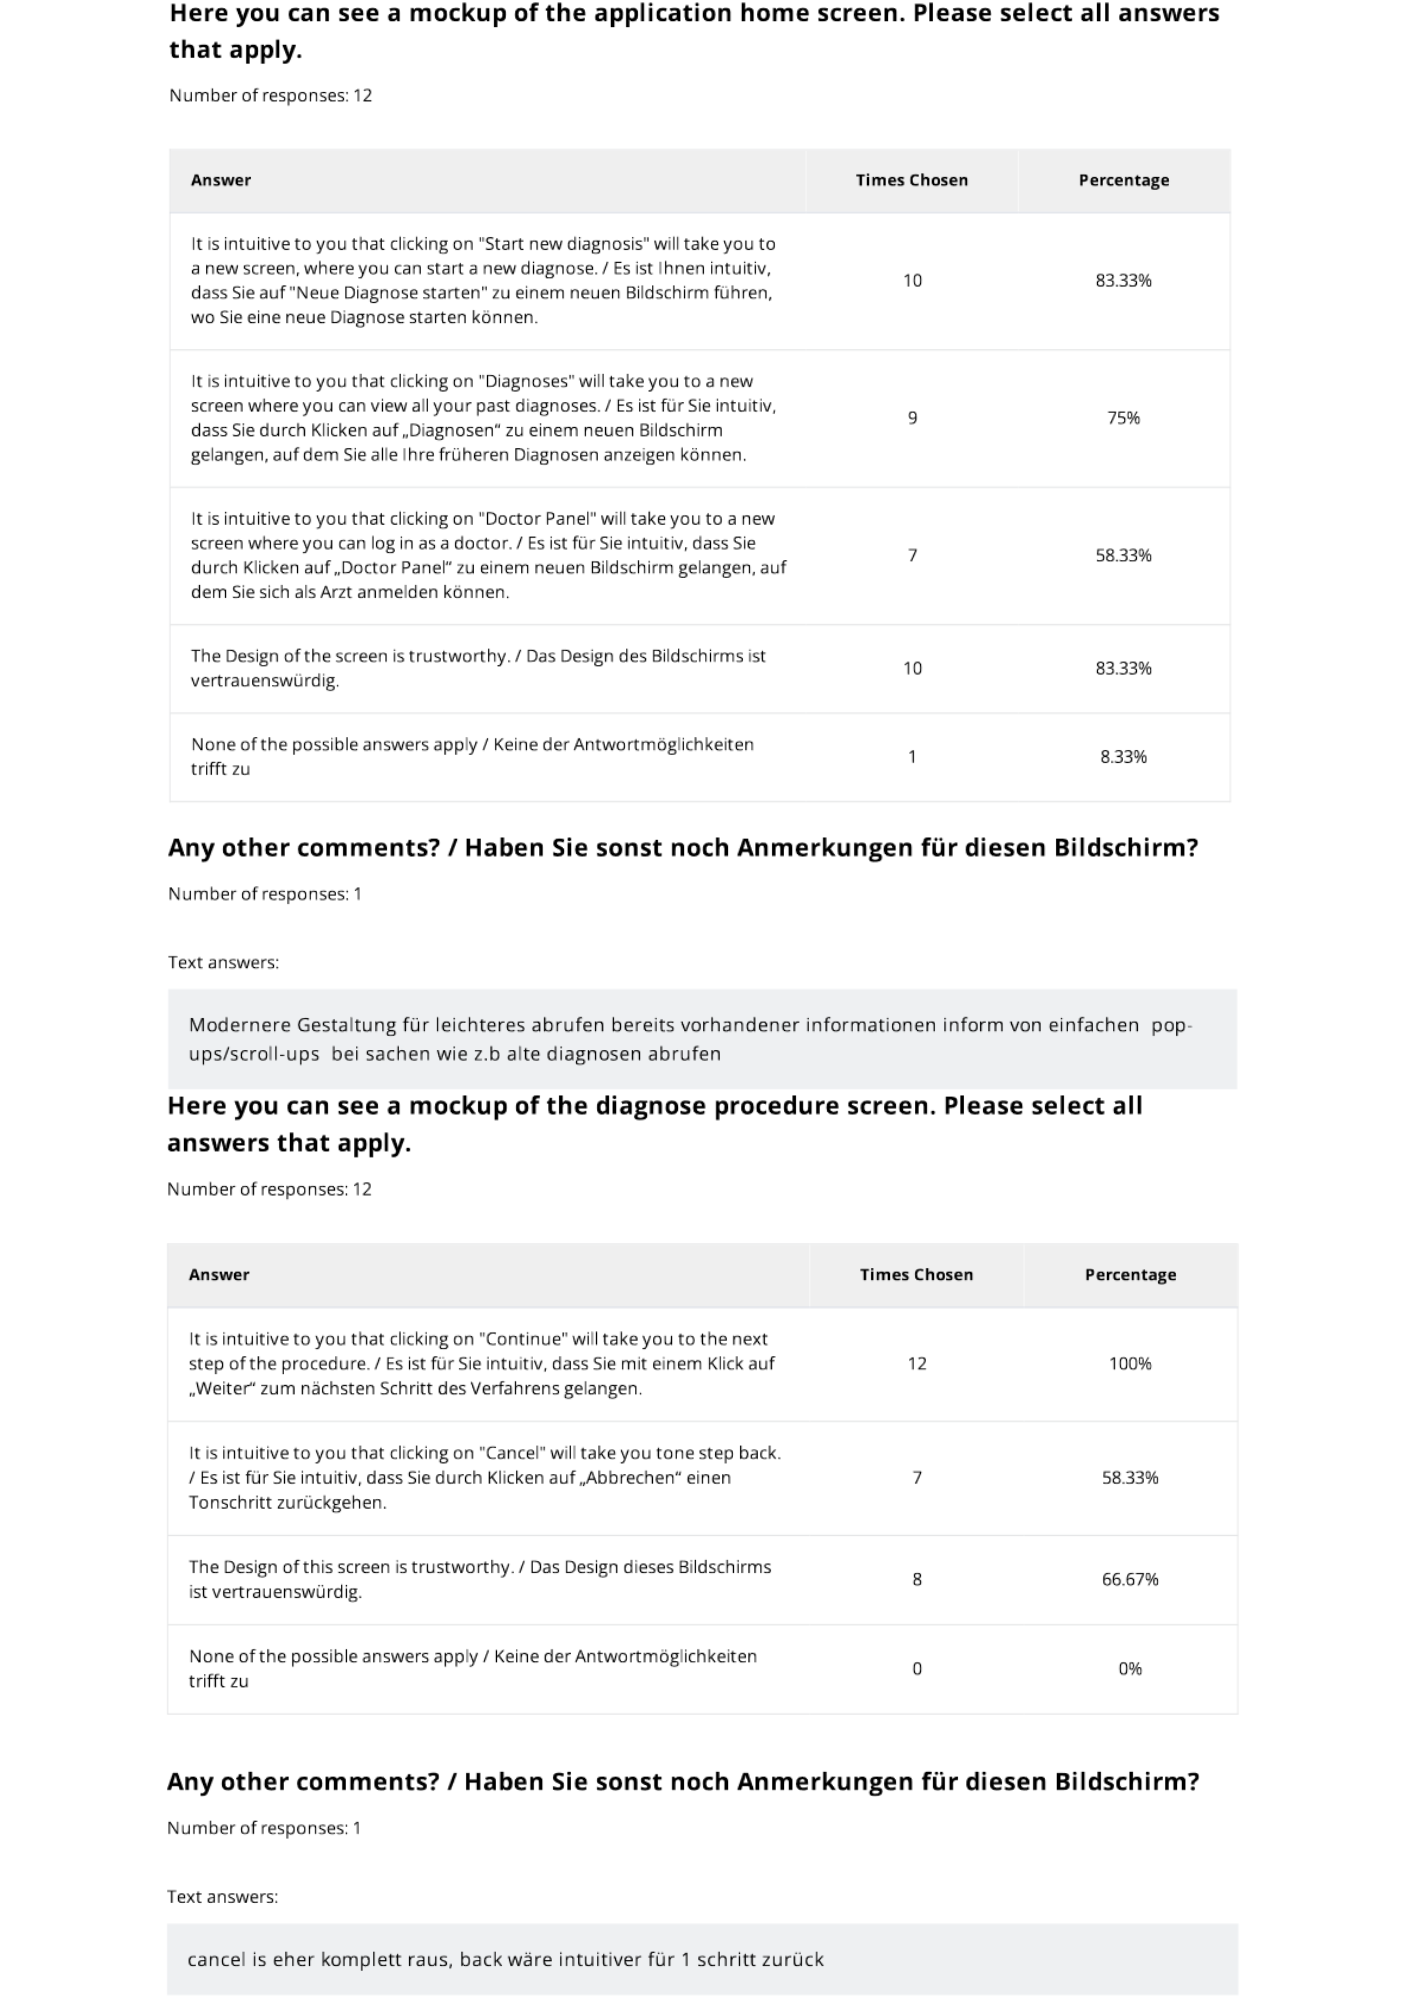
\includegraphics[scale=0.6]{umfrage21.png}
		\caption{Survey 2, Questions 1 - 4}
	\end{figure}
	\begin{figure}[H]
		\centering
		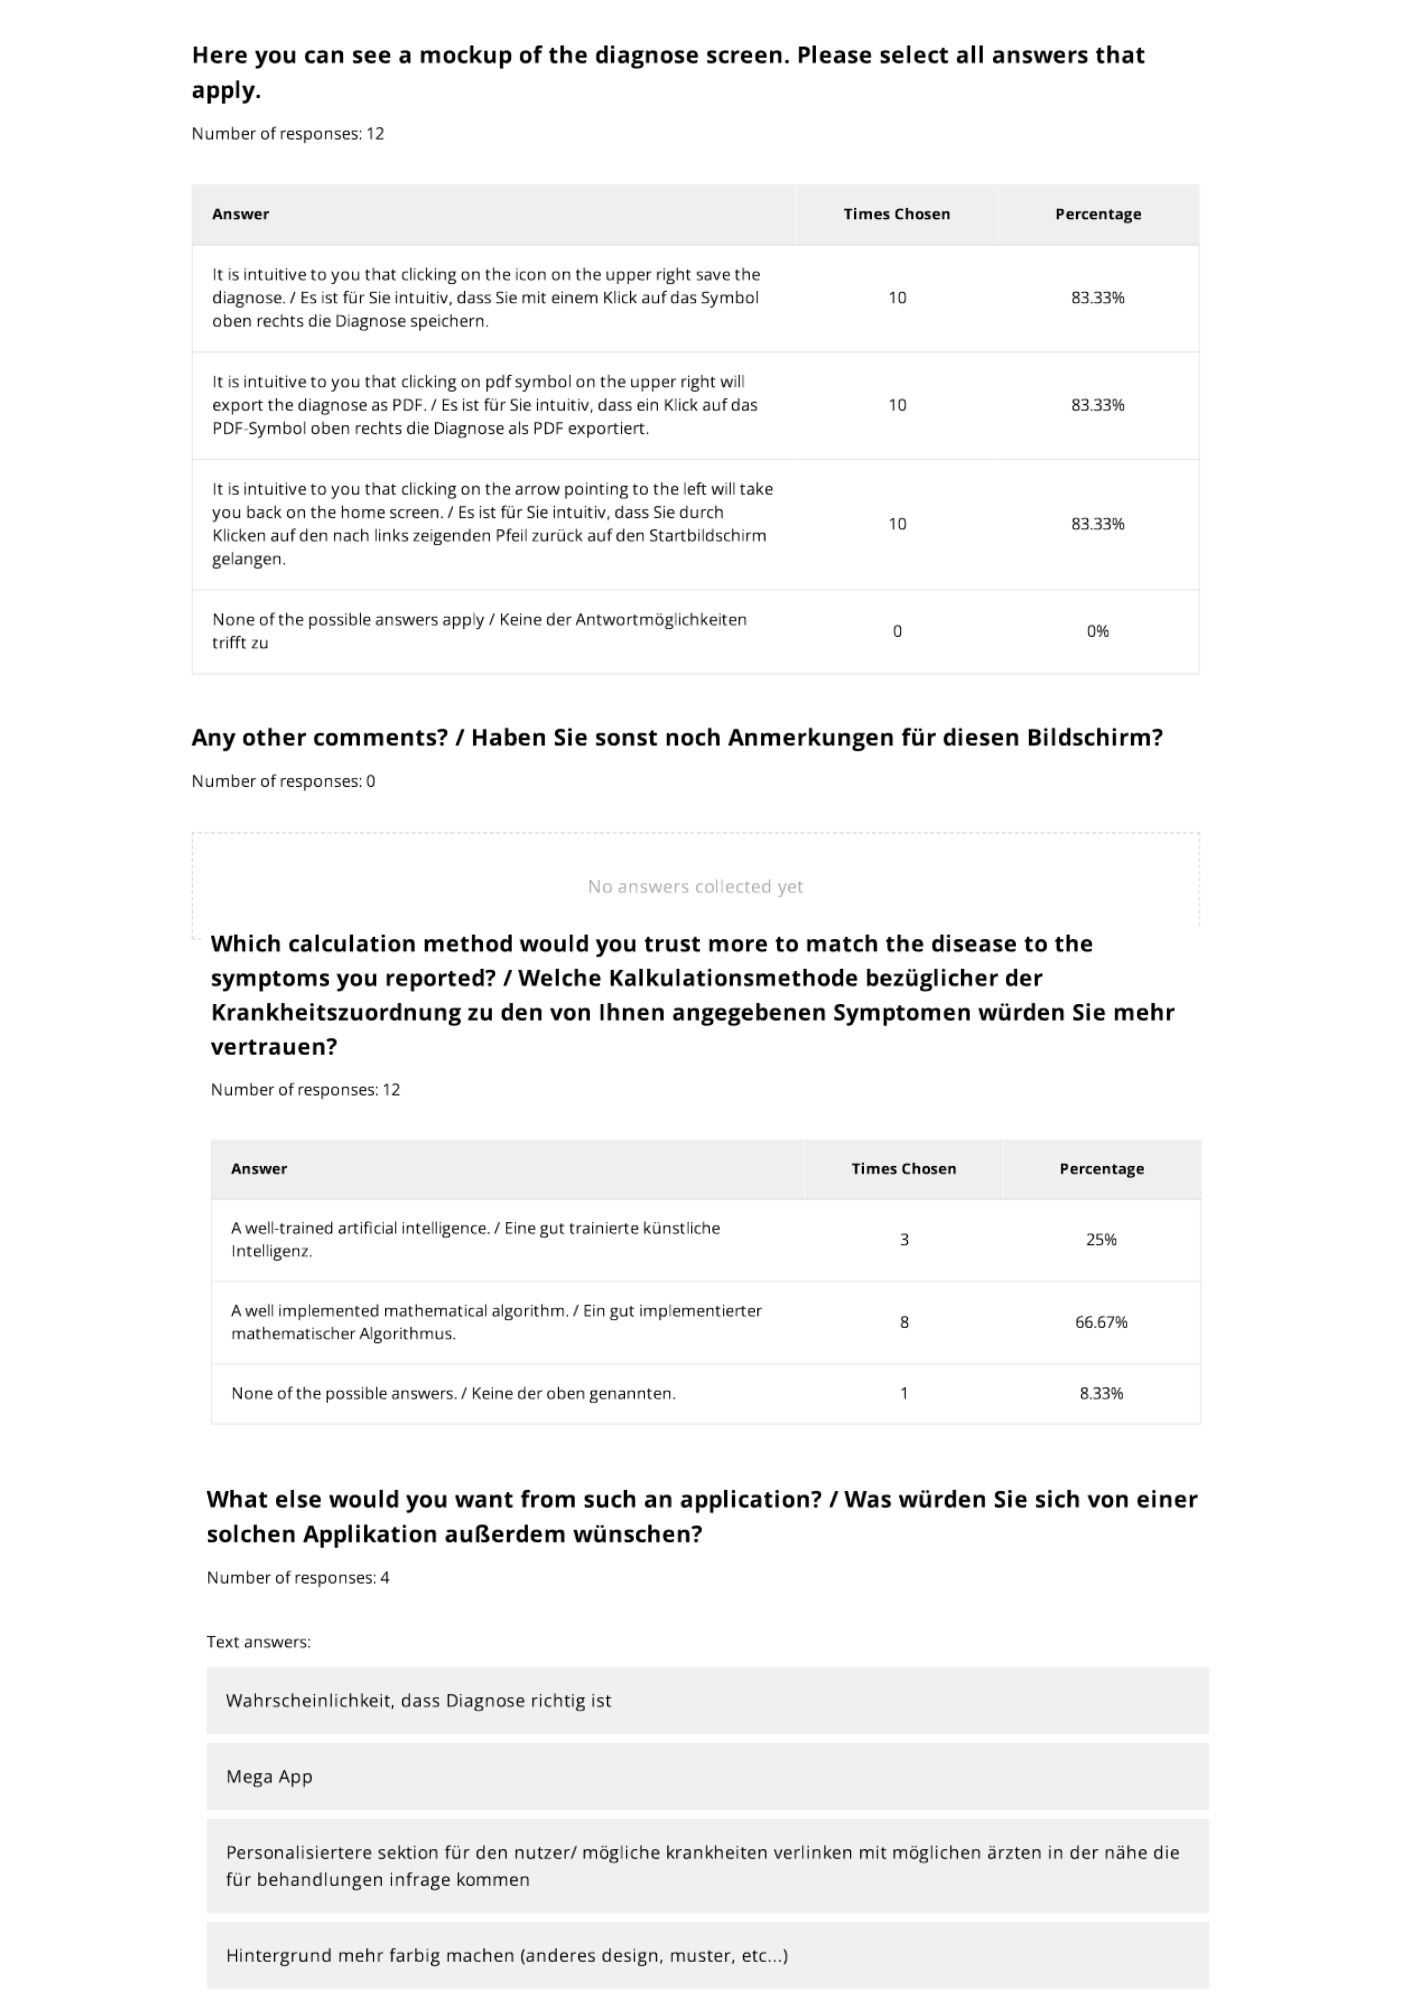
\includegraphics[scale=0.7]{umfrage22.png}
		\caption{Survey 2, Question 5 - 8}
	\end{figure}
\end{center}
\pagebreak


\tocless\chapter{Mock-ups}
\tocless\section{Home Screen}
\begin{figure}[H]
	\centering
	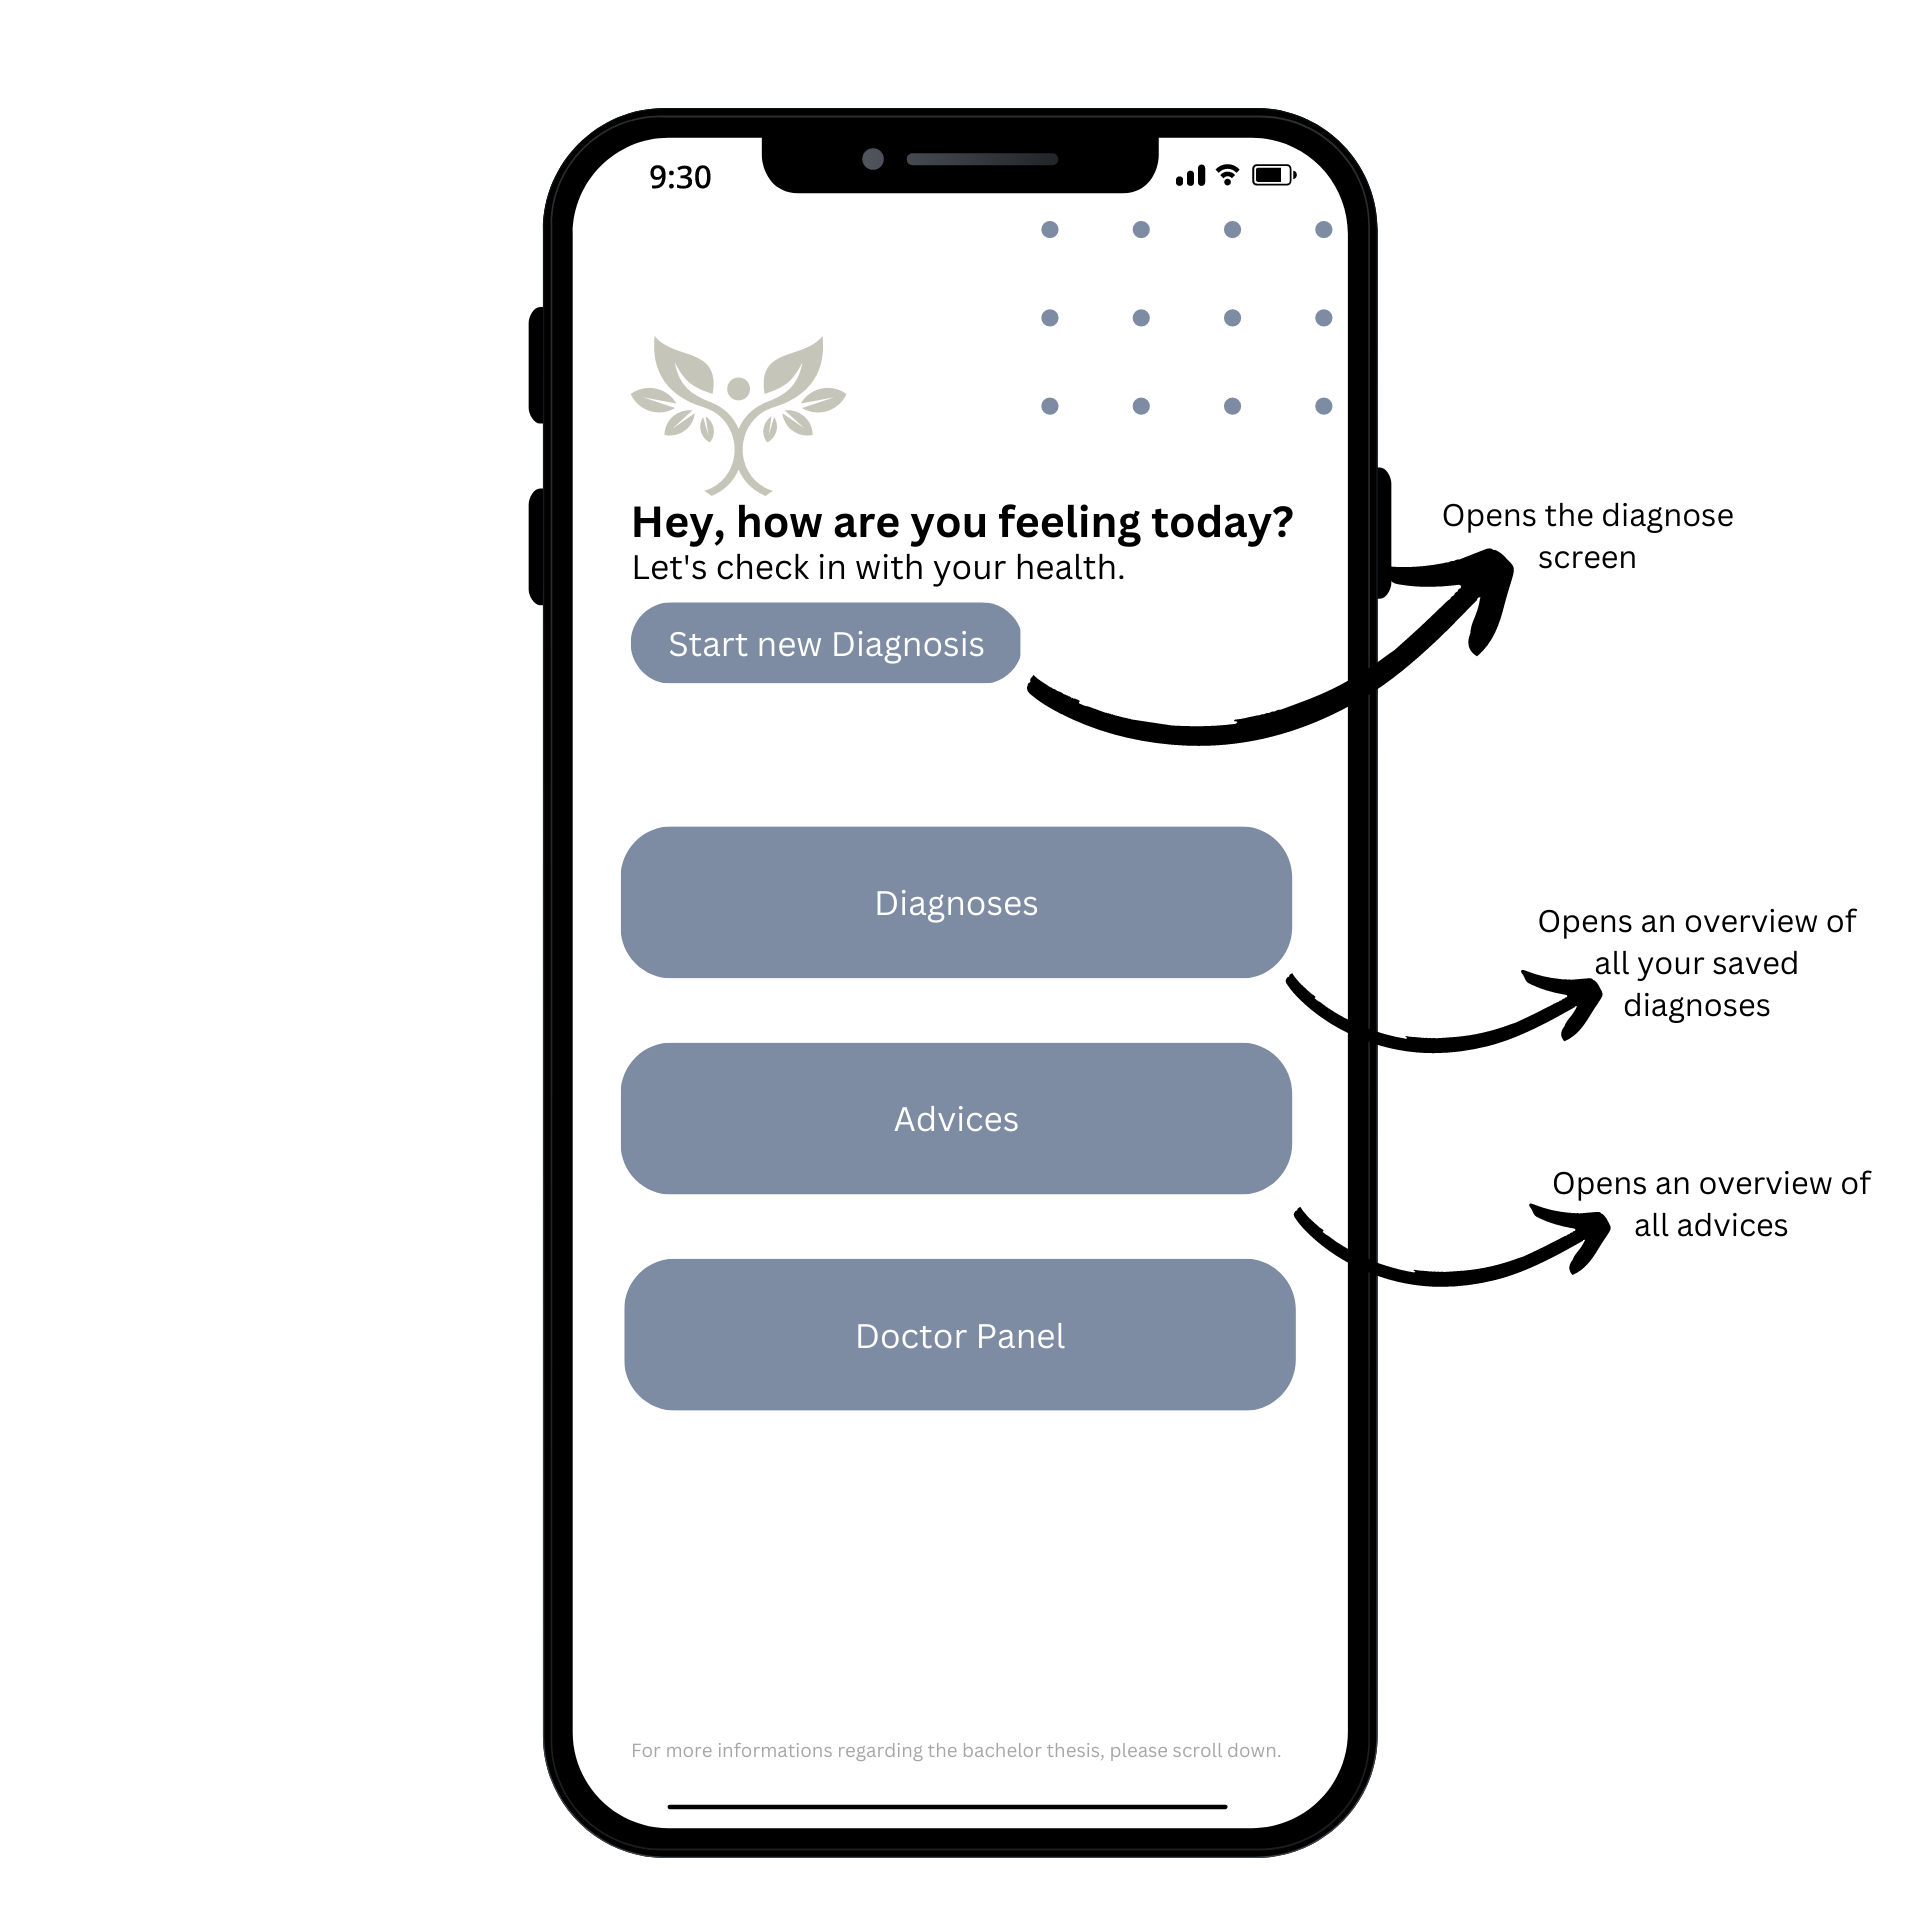
\includegraphics[scale=0.15]{home.png}
	\caption{Mock-up Home Screen}
\end{figure}

\tocless\section{Diagnostic Process Screen}
\begin{figure}[H]
	\centering
	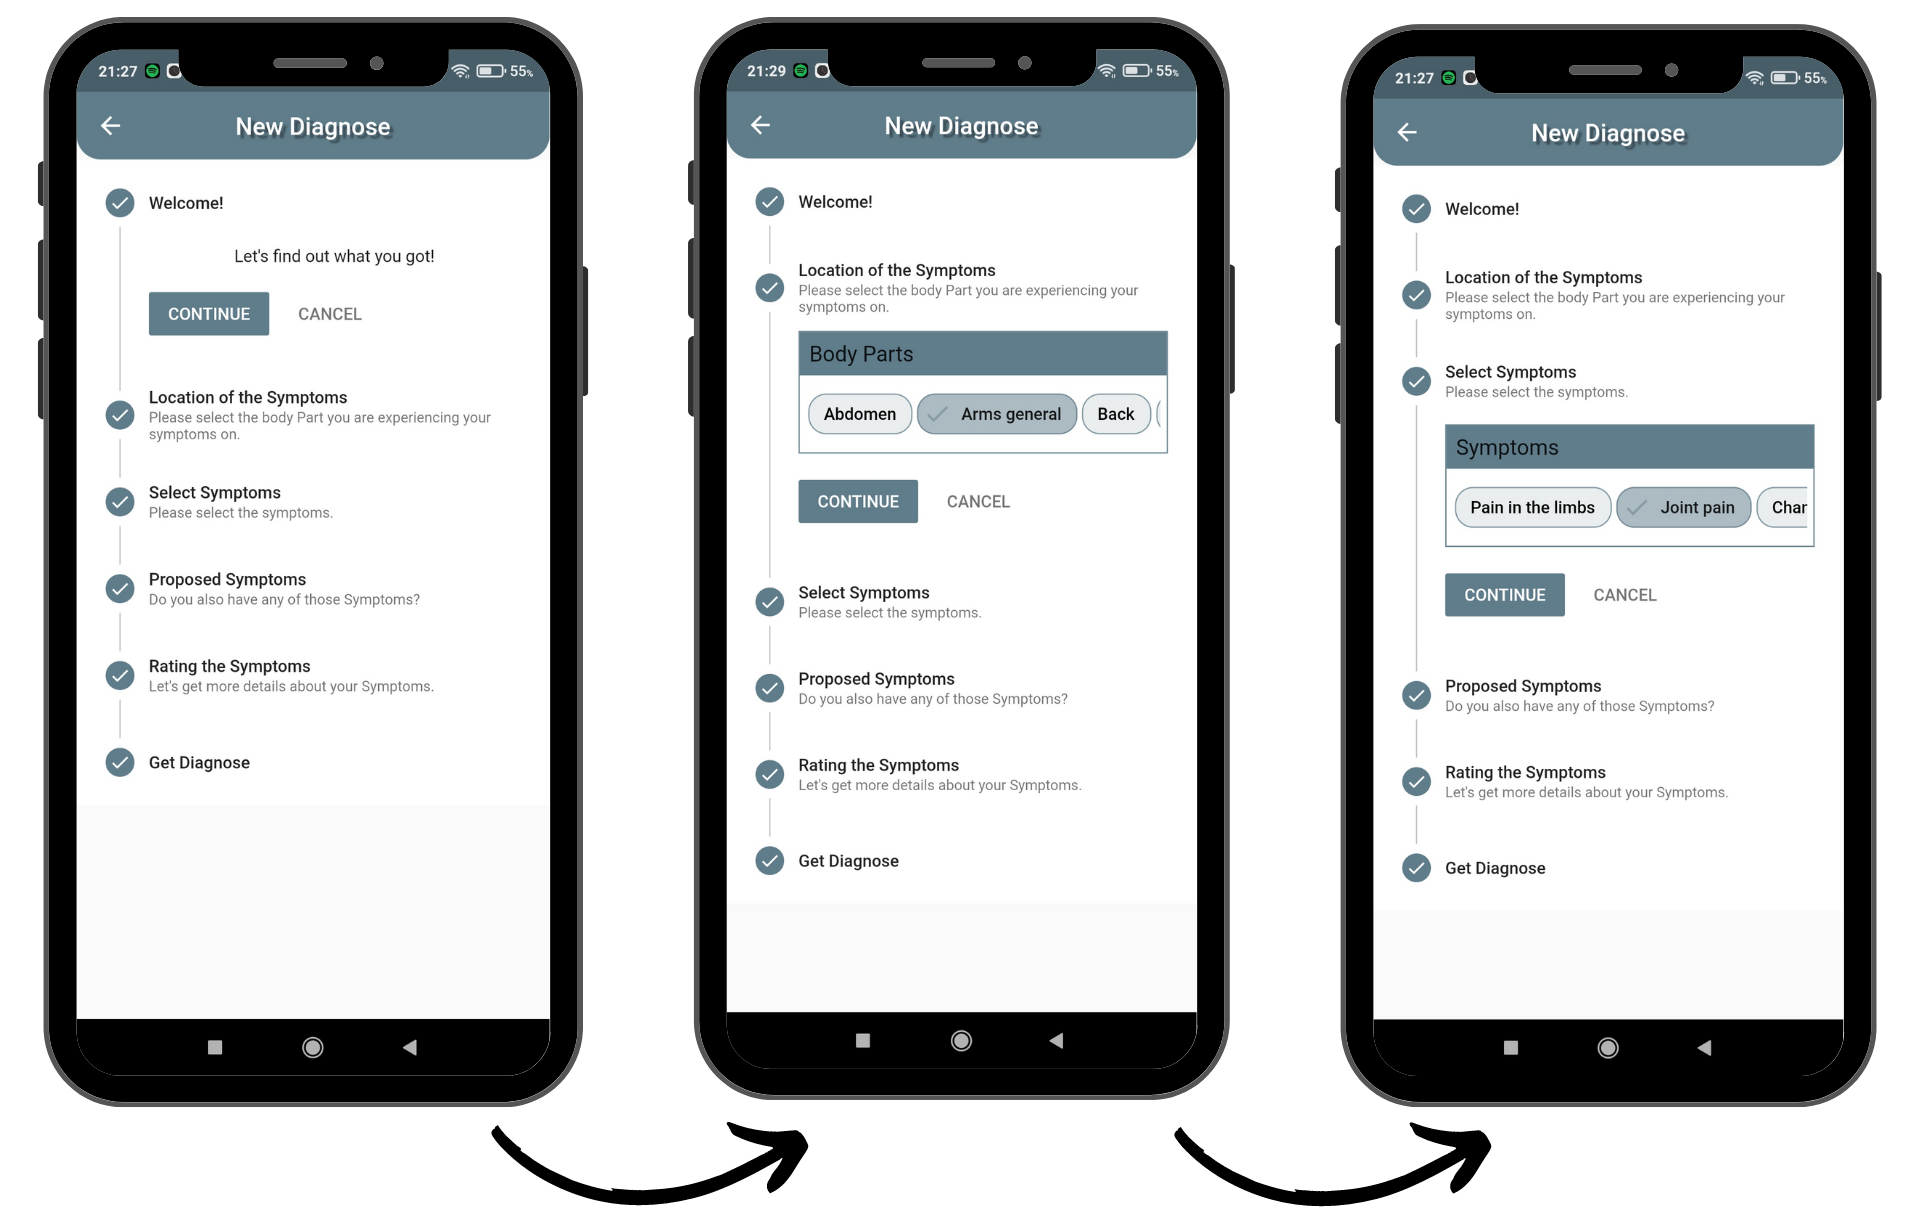
\includegraphics[scale=0.2]{diagnostic.png}
	\caption{Mock-up Diagnostic Process Screen}
\end{figure}

\tocless\section{Diagnose Screen}
\begin{figure}[H]
	\centering
	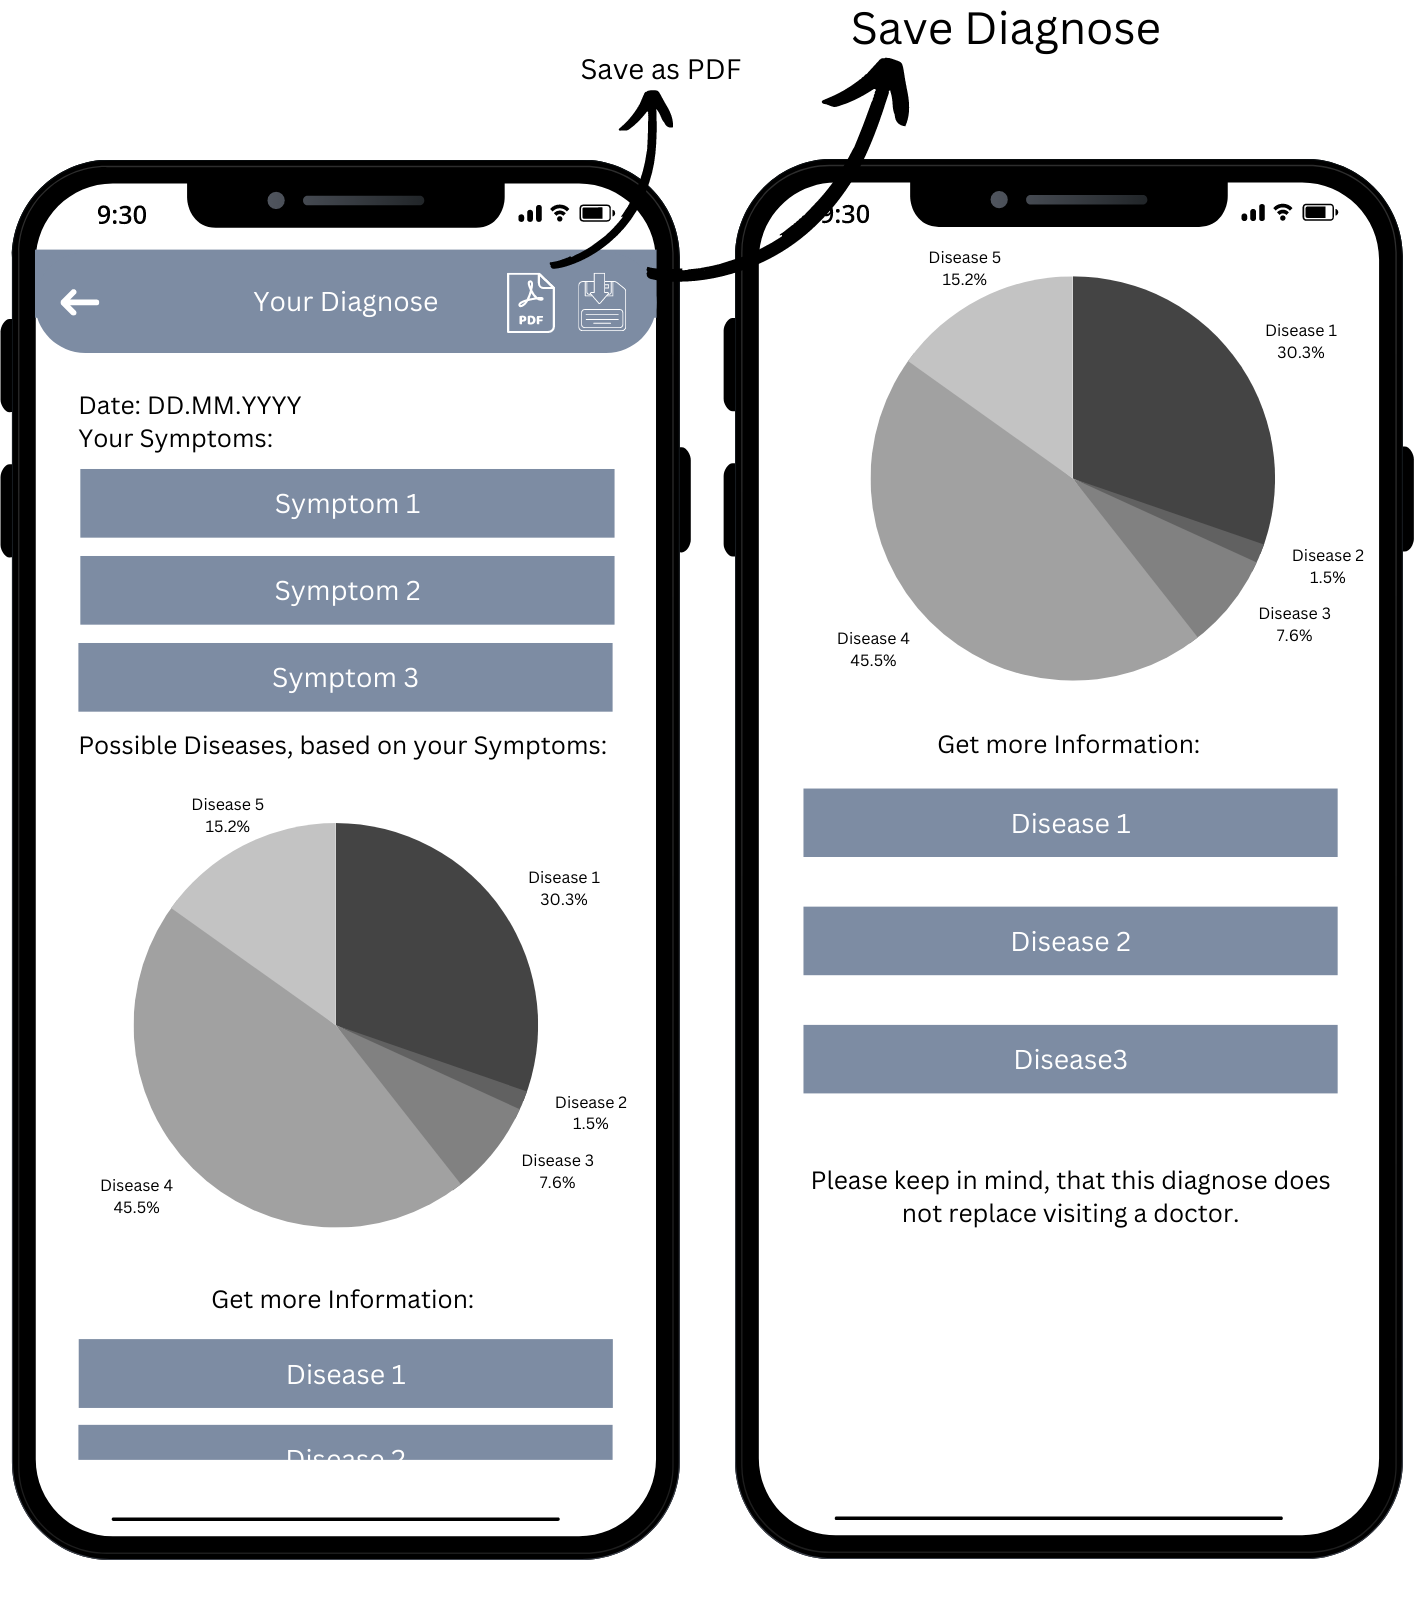
\includegraphics[scale=0.2]{diagnose.png}
	\caption{Mock-up Diagnose Screen}
\end{figure}

\tocless\section{Diagnose Overview Screen}
\begin{figure}[H]
	\centering
	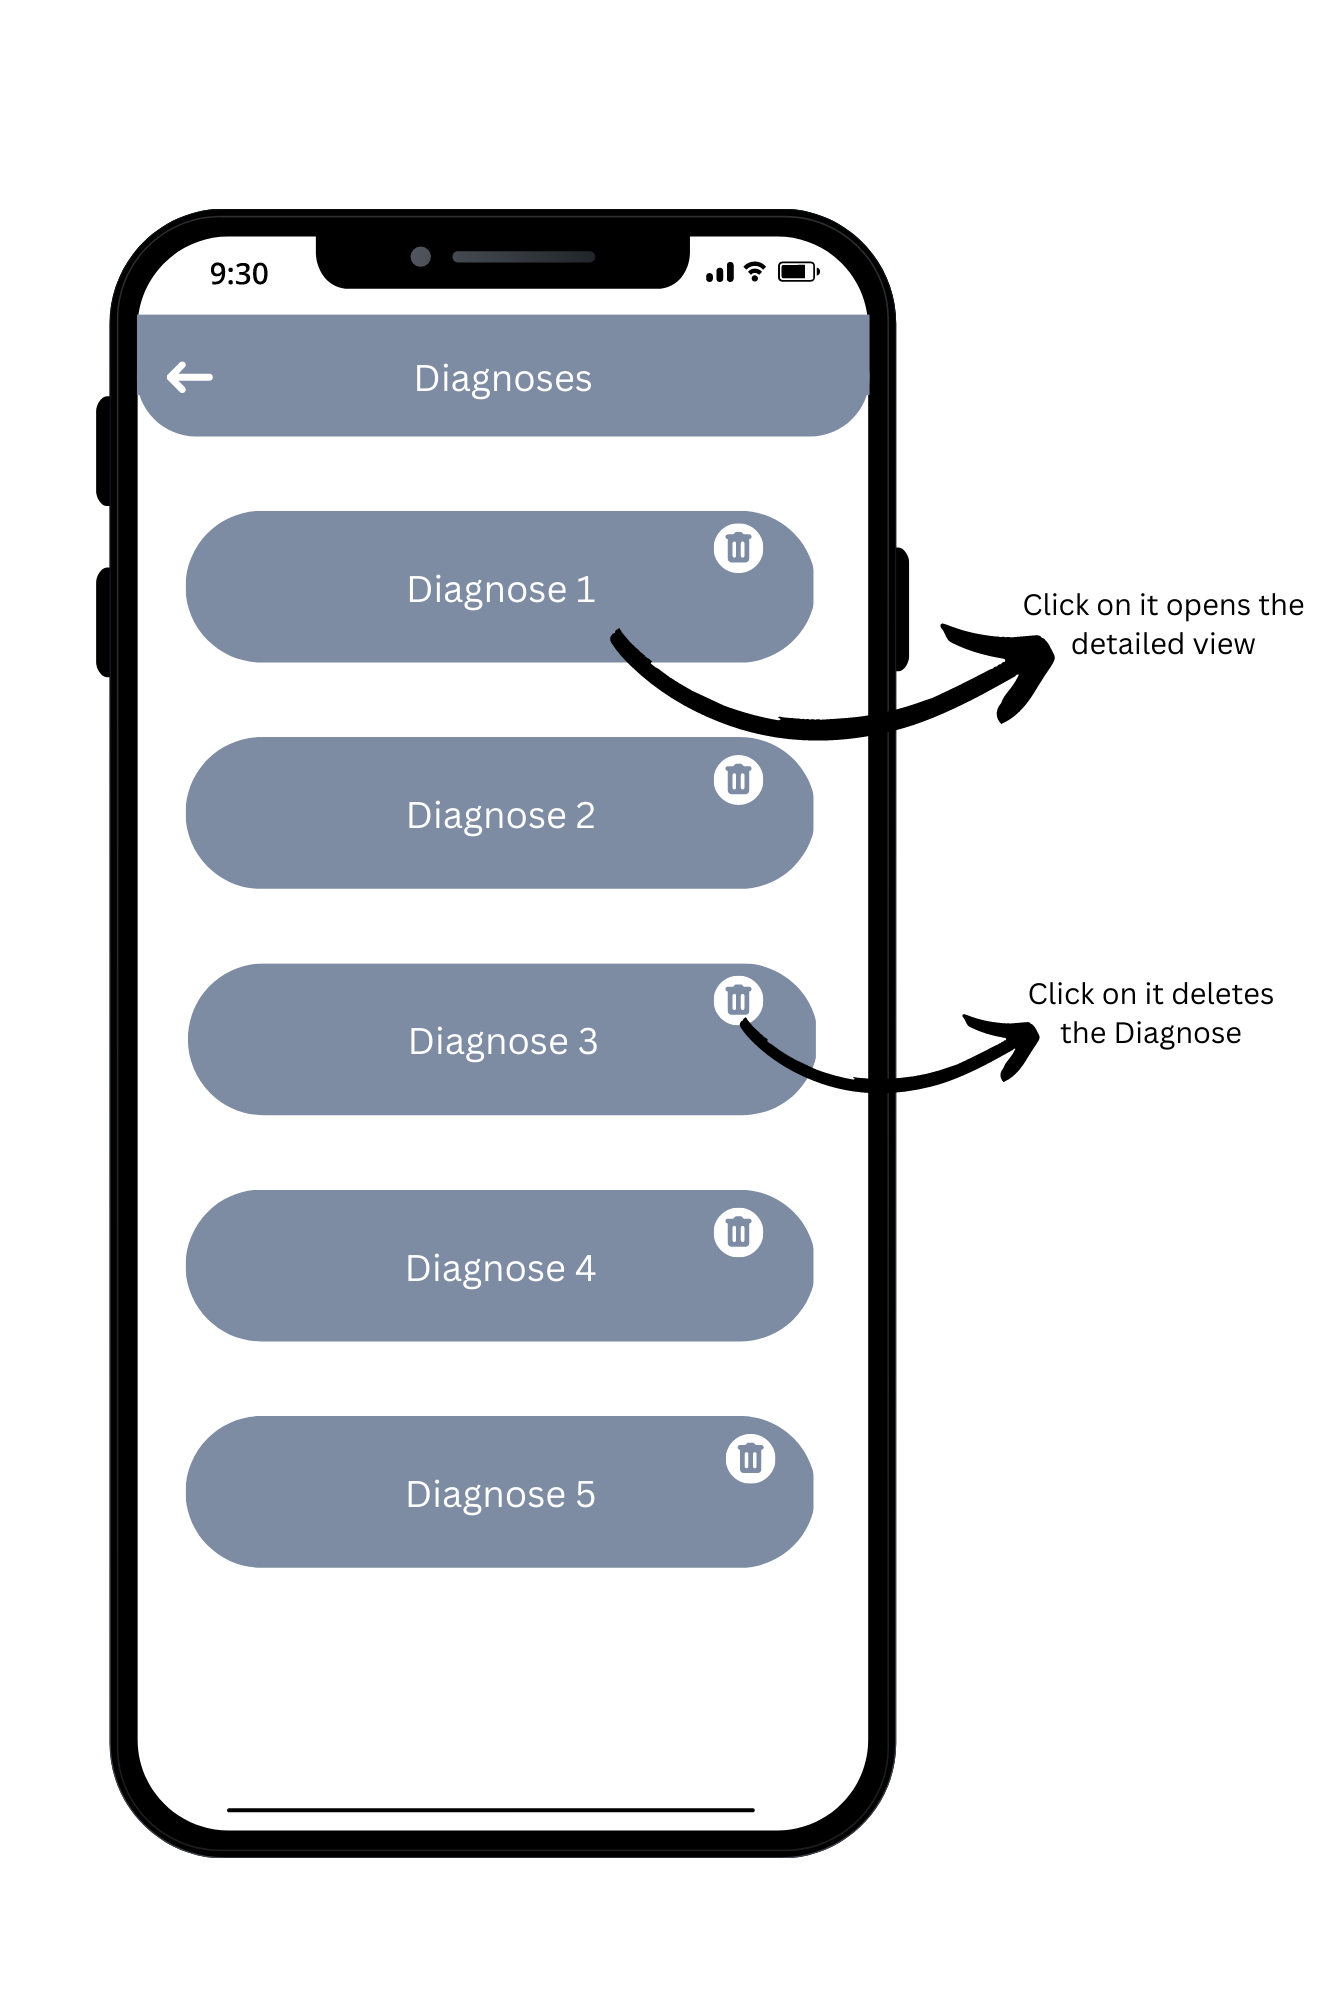
\includegraphics[scale=0.175]{6.png}
	\caption{Mock-up Diagnose Overview Screen}
\end{figure}

\tocless\section{Advice Overview Screen}
\begin{figure}[H]
	\centering
	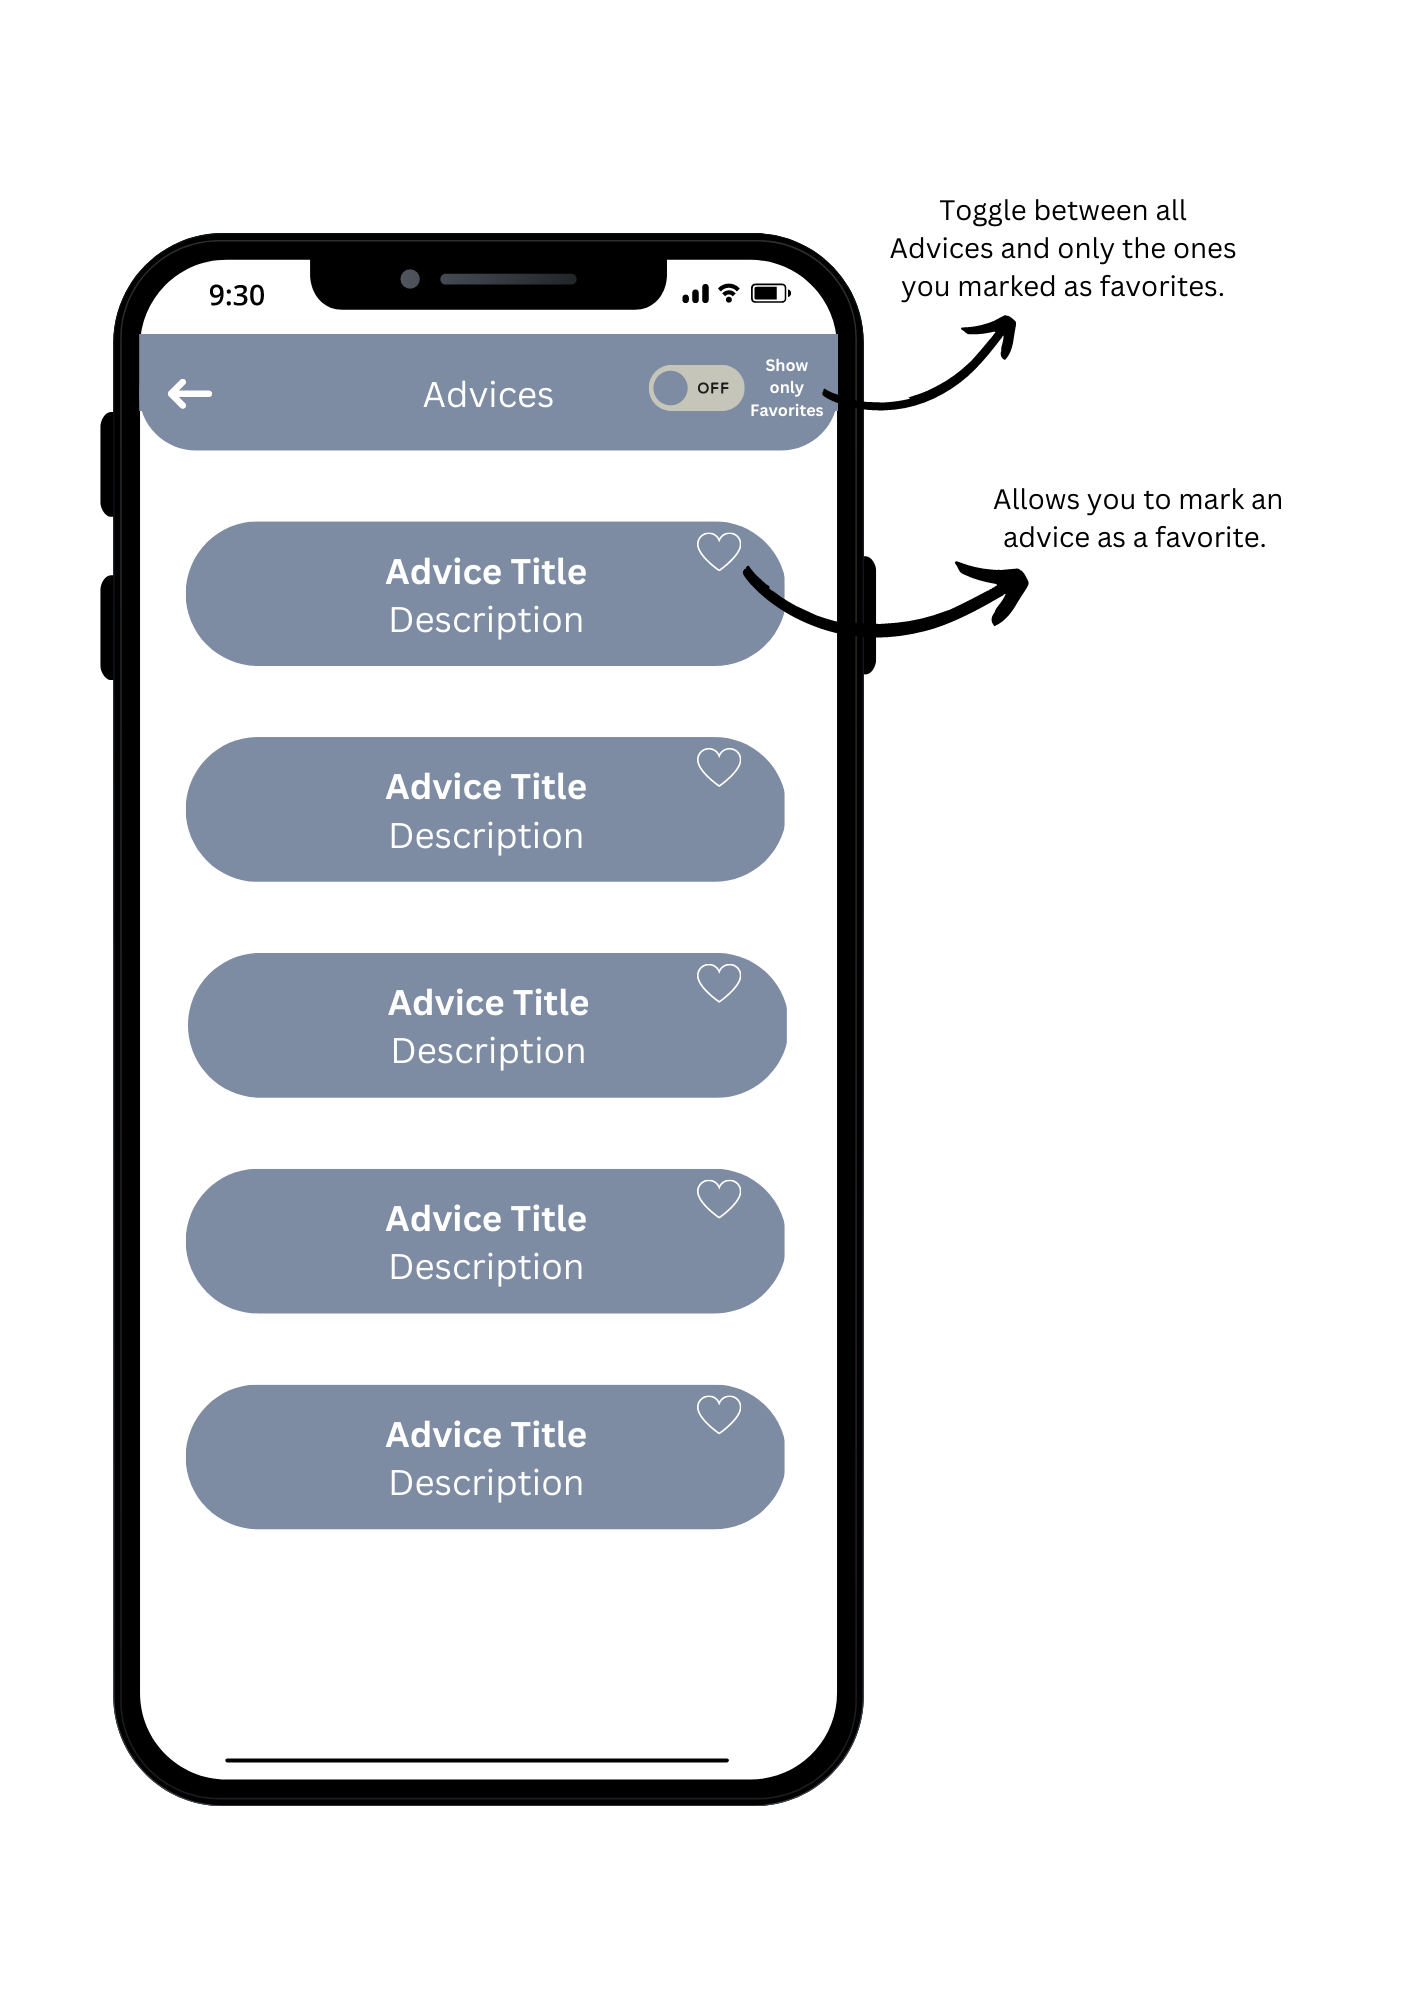
\includegraphics[scale=0.3]{7.png}
	\caption{Mock-up Advice Screen}
\end{figure}

\tocless\section{Login Screen}
\begin{figure}[H]
	\centering
	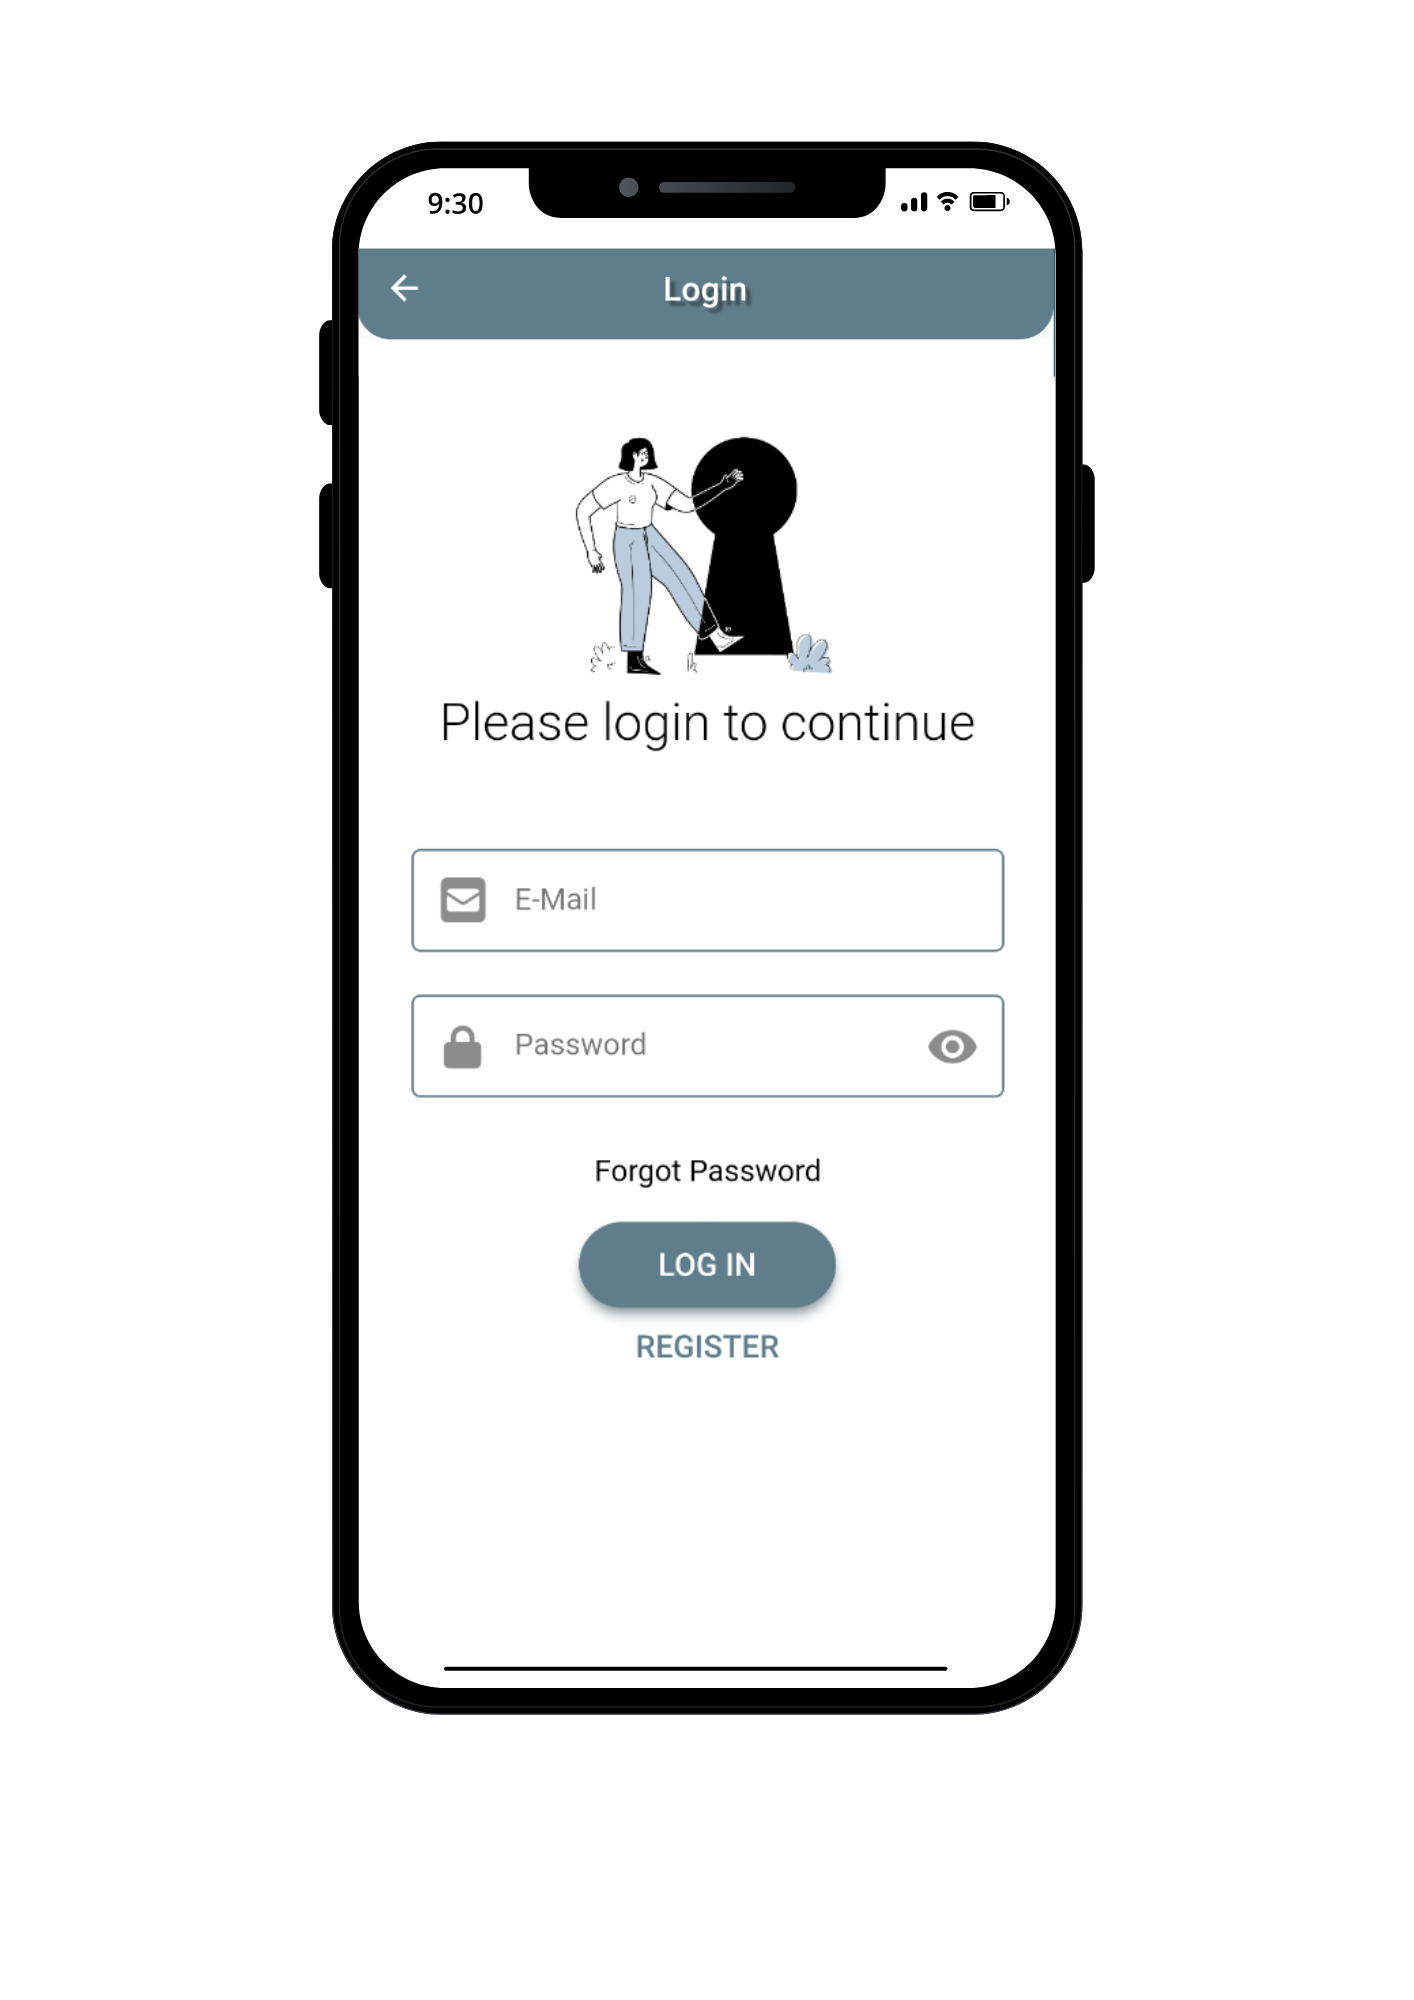
\includegraphics[scale=0.3]{login.png}
	\caption{Mock-up Login Screen}
\end{figure}

\tocless\section{Doctor Panel Screen}
\begin{figure}[H]
	\centering
	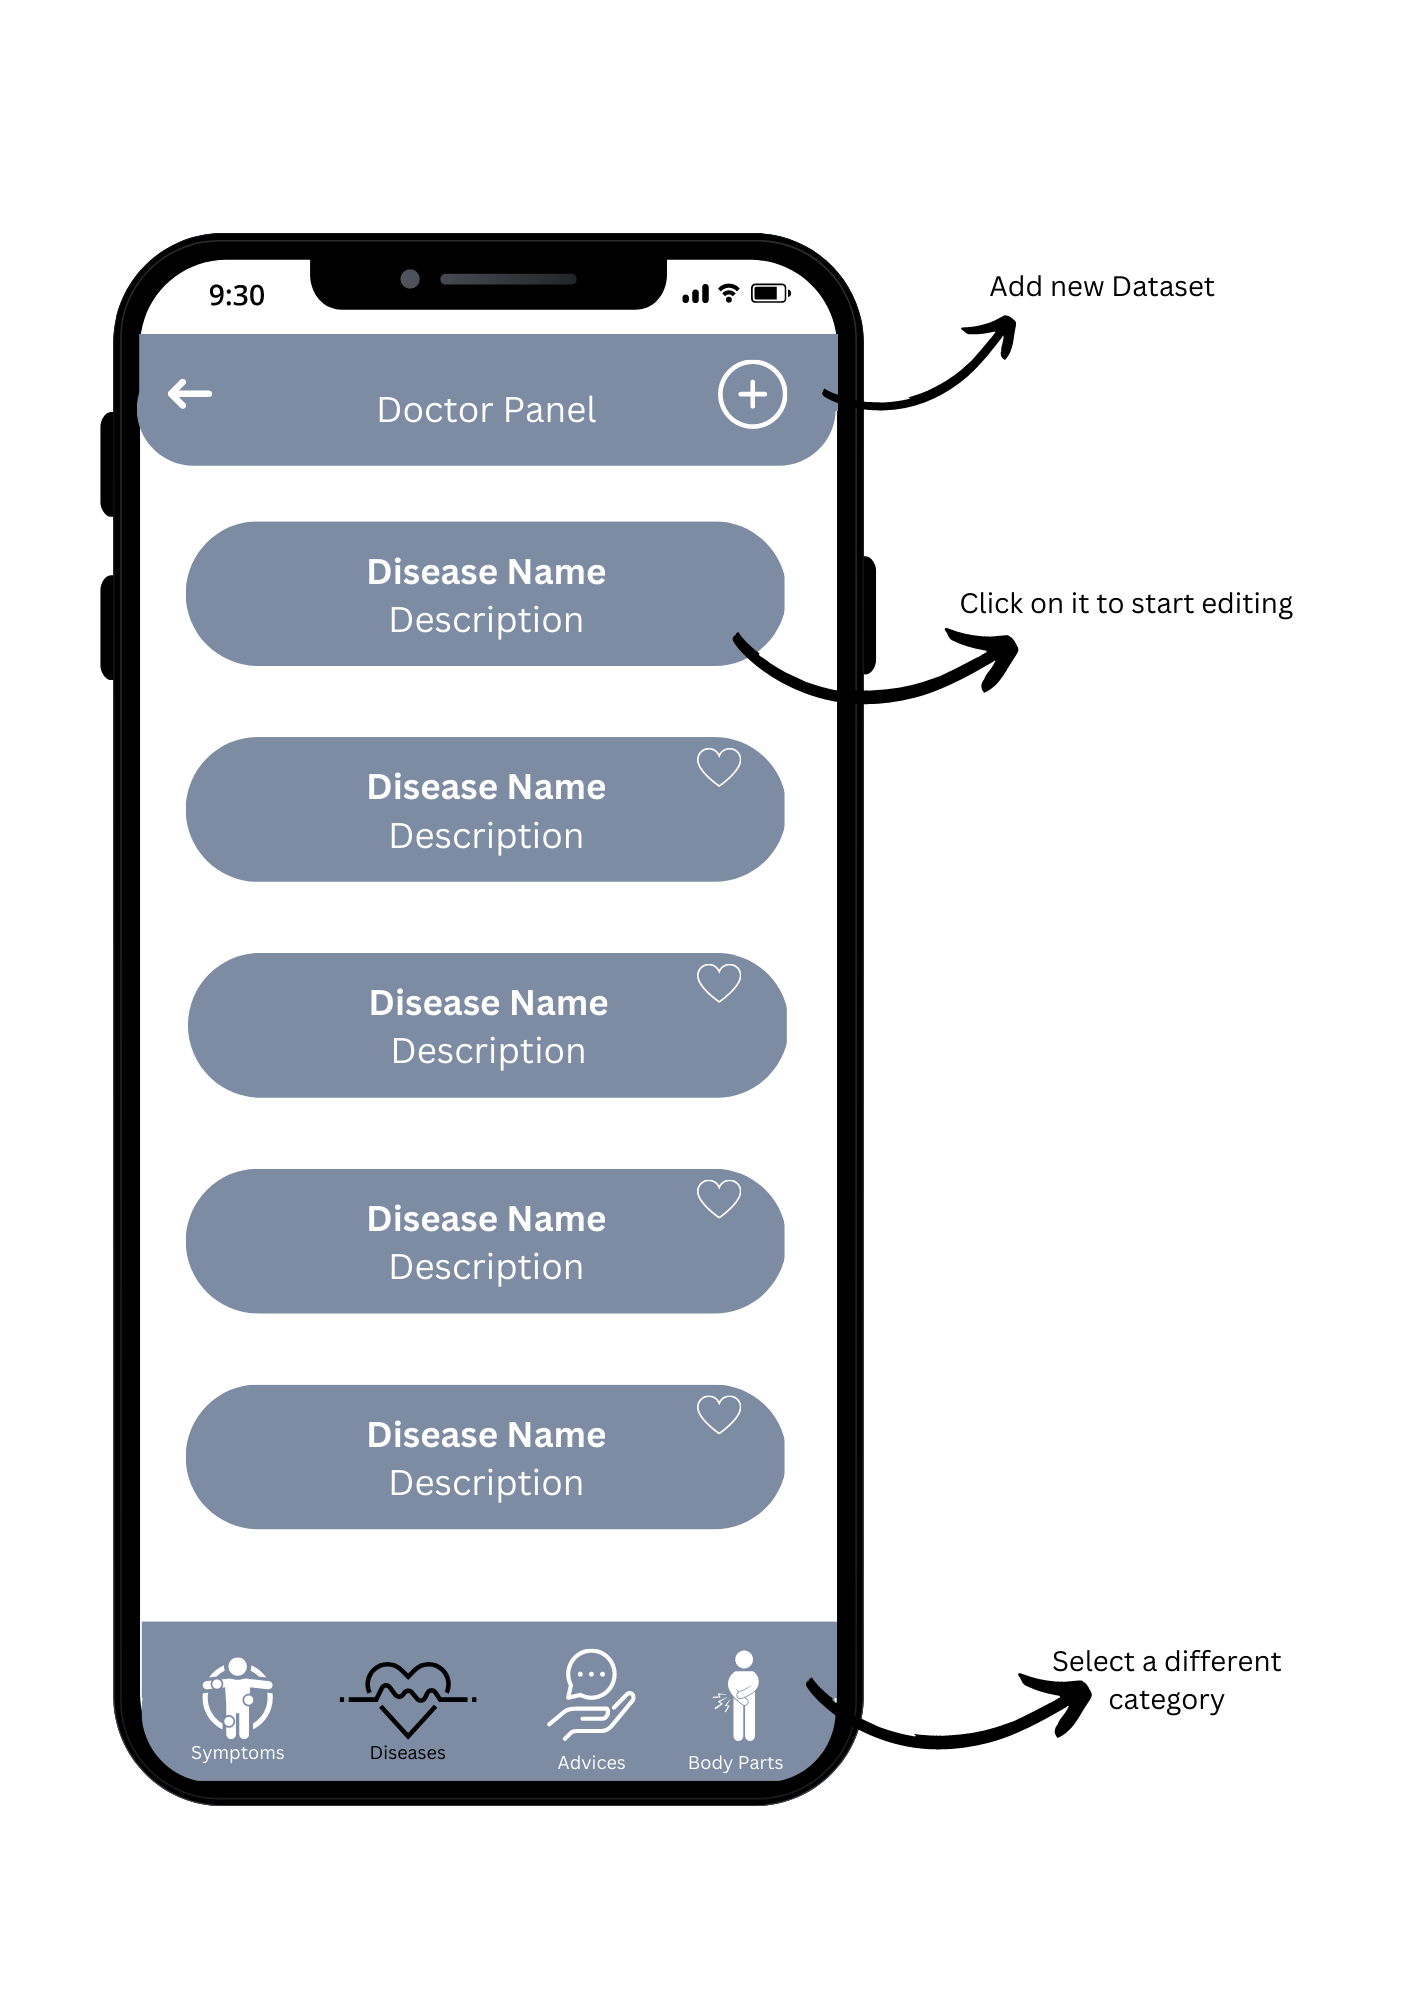
\includegraphics[scale=0.35]{8.png}
	\caption{Mock-up Doctor Panel}
\end{figure}



\tocless\chapter{Example Stepper Widget}
\begin{lstlisting}[caption=Stepper Example, basicstyle=\tiny]
	Widget build(BuildContext context) {
		return Scaffold(
		appBar: AppBarWidget(
			stringTitle: "New Diagnose",
			route: Routes.home,),
		body: Container(
		color: Colors.white,
		child: Theme(
			data: ThemeData(
			colorScheme: Theme.of(context).colorScheme.copyWith(
			primary: AppVariables.lightBlue,),),
		child: Stepper(
			type: stepperType,
			physics: ScrollPhysics(),
			currentStep: _currentStep,
			onStepTapped: (step) => tapped(step),
			onStepContinue: continued,
			onStepCancel: cancel,
			steps: [
			Step(
			title: const Text('Welcome!'),
			content: const Text("Let\'s find out what you got!"),
			isActive: _currentStep >= 0,
			state:
			_currentStep >= 0 ? StepState.complete : StepState.disabled,
			),
			Step(
			title: const Text('Location of the Symptoms'),
			subtitle: const Text(
			"Please select the body Part you are experiencing your symptoms on.",),
			content: MultiSelectChipField<String>(
			items: allbodyParts,
			icon: Icon(Icons.check),
			headerColor: AppVariables.lightBlue,
			decoration: BoxDecoration(
			border: Border.all(
			color: AppVariables.lightBlue,
			),),
			selectedChipColor: AppVariables.lightBlue.withOpacity(0.5),
			title: const Text("Body Parts"),
			textStyle: const TextStyle(color: Colors.black),
			chipColor: AppVariables.lightBlue.withOpacity(0.1),
			onTap: (values) {
				setState(() {
					selectedBodyParts = values;
				});},),
			isActive: _currentStep >= 0,
			state:
			_currentStep >= 0 ? StepState.complete : StepState.disabled,),
			Step(
			title: const Text('Select Symptoms'),
			subtitle: const Text(
			"Please select the symptoms.",
			),
			content: MultiSelectChipField<String>(
			items: allSymptomsOfBodyPart,
			icon: Icon(Icons.check),
			headerColor: AppVariables.lightBlue,
			decoration: BoxDecoration(
			border: Border.all(
			color: AppVariables.lightBlue,
			),),
			selectedChipColor: AppVariables.lightBlue.withOpacity(0.5),
			title: const Text("Symptoms"),
			textStyle: const TextStyle(color: Colors.black),
			chipColor: AppVariables.lightBlue.withOpacity(0.1),
			onTap: (values) {
				setState(() {
					selectedSymptoms = values;
				});},),
			isActive: _currentStep >= 0,
			state:
			_currentStep >= 0 ? StepState.complete : StepState.disabled,),
...
\end{lstlisting}
\pagebreak

\tocless\chapter{Implemented Services}
\tocless\section{DatabaseService}
\begin{lstlisting}[caption=DatabaseService Code]
class DatabaseService {
	/* CREATE AN INSTANCE OF THE DATABASE */
	DatabaseService._();
	static DatabaseService _instance = DatabaseService._();
	static DatabaseService get instance => _instance;
	
	/* GET REFERENCES */
	final CollectionReference _bodyPartReference =
	FirebaseFirestore.instance.collection('body_parts');
	
	final CollectionReference _symptomCollectionReference =
	FirebaseFirestore.instance.collection('symptoms');
	
	final CollectionReference _diseasesCollectionReference =
	FirebaseFirestore.instance.collection('diseases');
	
	final CollectionReference _adviceCollectionReference =
	FirebaseFirestore.instance.collection('advices');
	
	final CollectionReference _doctorCollectionReference =
	FirebaseFirestore.instance.collection('doctors');
	/* GET BODY PART DATA */
	getAllBodyParts() {
		return _bodyPartReference.snapshots();
	}
	
	Future<List<BodyPart>> retrieveBodyParts() async {
		QuerySnapshot<Map<String, dynamic>> snapshot =
		await _bodyPartReference.get() as QuerySnapshot<Map<String, dynamic>>;
		return snapshot.docs
		.map((docSnapshot) => BodyPart.fromDocumentSnapshot(docSnapshot))
		.toList();
	}

// MORE METHODS 
...
\end{lstlisting}
\pagebreak
\tocless\section{ConvertService}
\begin{lstlisting}[caption=AppNavigator Class]
class ConvertService {
	/* CREATE AN INSTANCE OF THE DATABASE */
	ConvertService._();
	static ConvertService _instance = ConvertService._();
	static ConvertService get instance => _instance;
	
	// SYMPTOMS
	Future<List<MultiSelectItem<String>>> getAllSymptoms() async {
		var data = await DatabaseService.instance.retrieveSymptoms();
		List<MultiSelectItem<String>> symptoms = [];
		for (var element in data) {
			symptoms.add(
			MultiSelectItem(element.name, element.name),
			);
		}
		return symptoms;
	}
// MORE METHODS
...
\end{lstlisting}
\pagebreak
\tocless\section{AppNavigator (NavigationService)}
\begin{lstlisting}[caption=AppNavigator Class]
	enum Routes { survey, home, advices, doctorPanel, detailScreen, diagnosesList }
	
	class _Paths {
		static const String survey = '/';
		static const String home = '/home';
		static const String advices = '/home/advices';
		static const String doctorPanel = '/home/doctorPanel';
		static const String detailScreen = '/home/detailScreen';
		static const String diagnosesList = '/home/items';
		
		static const Map<Routes, String> _pathMap = {
			Routes.home: _Paths.home,
			Routes.survey: _Paths.survey,
			Routes.advices: _Paths.advices,
			Routes.doctorPanel: _Paths.doctorPanel,
			Routes.detailScreen: _Paths.detailScreen,
			Routes.diagnosesList: _Paths.diagnosesList
		};
		
		static String of(Routes route) => _pathMap[route] ?? survey;
	}
	
	class AppNavigator {
		static GlobalKey<NavigatorState> navigatorKey = GlobalKey();
		static Route onGenerateRoute(RouteSettings settings) {
			switch (settings.name) {
				case _Paths.survey:
				return FadeRoute(page: SurveyScreenFlutter());
				case _Paths.advices:
				return FadeRoute(page: AdviceScreen());
				case _Paths.doctorPanel:
				return FadeRoute(
				page: FirebaseAuth.instance.currentUser != null
				? DoctorPanelScreen(title: "DoctorPanel")
				: LoginScreen(),
				);
				case _Paths.detailScreen:
				return FadeRoute(page: DetailScreen(null));
				case _Paths.diagnosesList:
				return FadeRoute(page: DiagnosesScreen());
				case _Paths.home:
				default:
				return FadeRoute(page: HomeScreen());
			}
		}
		
		static Future? push<T>(Routes route, [T? arguments]) =>
		state?.pushNamed(_Paths.of(route), arguments: arguments);
		static Future? replaceWith<T>(Routes route, [T? arguments]) =>
		state?.pushReplacementNamed(_Paths.of(route), arguments: arguments);
		static void pop() => state?.pop();
		static NavigatorState? get state => navigatorKey.currentState;
	}
\end{lstlisting}

\pagebreak
\tocless\section{AuthService}
\begin{lstlisting}[caption=AuthService]
class AuthService {
	/* CREATE AN INSTANCE OF THE DATABASE */
	AuthService._();
	static AuthService _instance = AuthService._();
	static AuthService get instance => _instance;
	
	FirebaseAuth auth = FirebaseAuth.instance;
	
	Future<String?> registration(SignupData pData) async {
		try {
			UserCredential userCredential =
			await FirebaseAuth.instance.createUserWithEmailAndPassword(
			email: pData.name!,
			password: pData.password!,
			);
			
			Doctor d = Doctor(
			email: pData.name!,
			createdSymptomsIDs: [],
			createdDiseasesIDs: [],
			createdAdvicesIDs: [],
			);
			
			DatabaseService.instance.addNewDoctor(
			FirebaseAuth.instance.currentUser!.uid,
			d.toMap(),
			);
			
			print(FirebaseAuth.instance.currentUser);
		} catch (e) {
			print(e);
		}
	}
	
	Future<String?> signIn(LoginData pData) async {
		try {
			UserCredential userCredential =
			await FirebaseAuth.instance.signInWithEmailAndPassword(
			email: pData.name,
			password: pData.password,
			);
		} on FirebaseAuthException catch (e) {
			if (e.code == 'user-not-found') {
				print('No user found for that email.');
			} else if (e.code == 'wrong-password') {
				print('Wrong password provided for that user.');
			}
		}
	}
// MORE METHODS
...
\end{lstlisting}
\tocless\chapter{Evaluation of the Algorithm}
\tocless\section{Information about the System}
\tocless\subsection{CPU}
\begin{figure}[H]
	\centering
	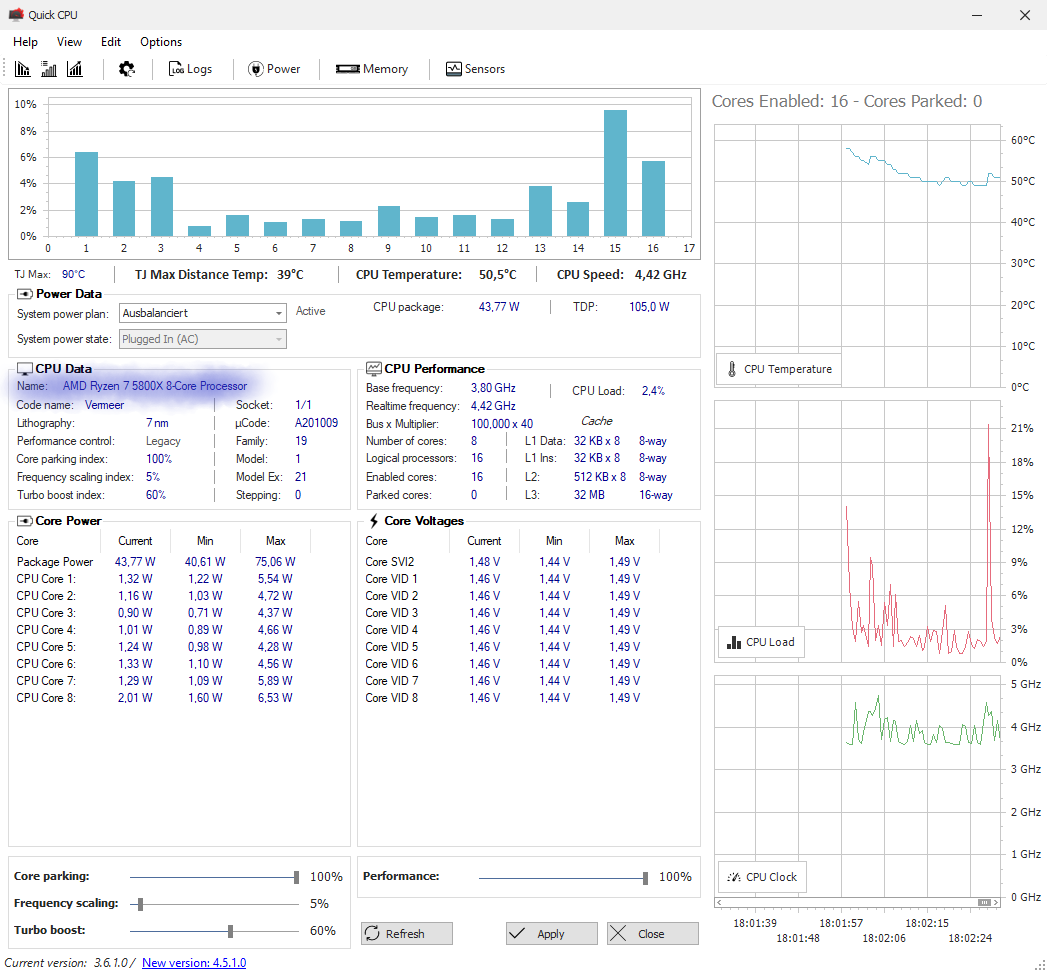
\includegraphics[scale=0.4]{cpu.png}
	\caption{System CPU Information}
\end{figure}
\tocless\subsubsection{Emulator}
\begin{figure}[H]
	\centering
	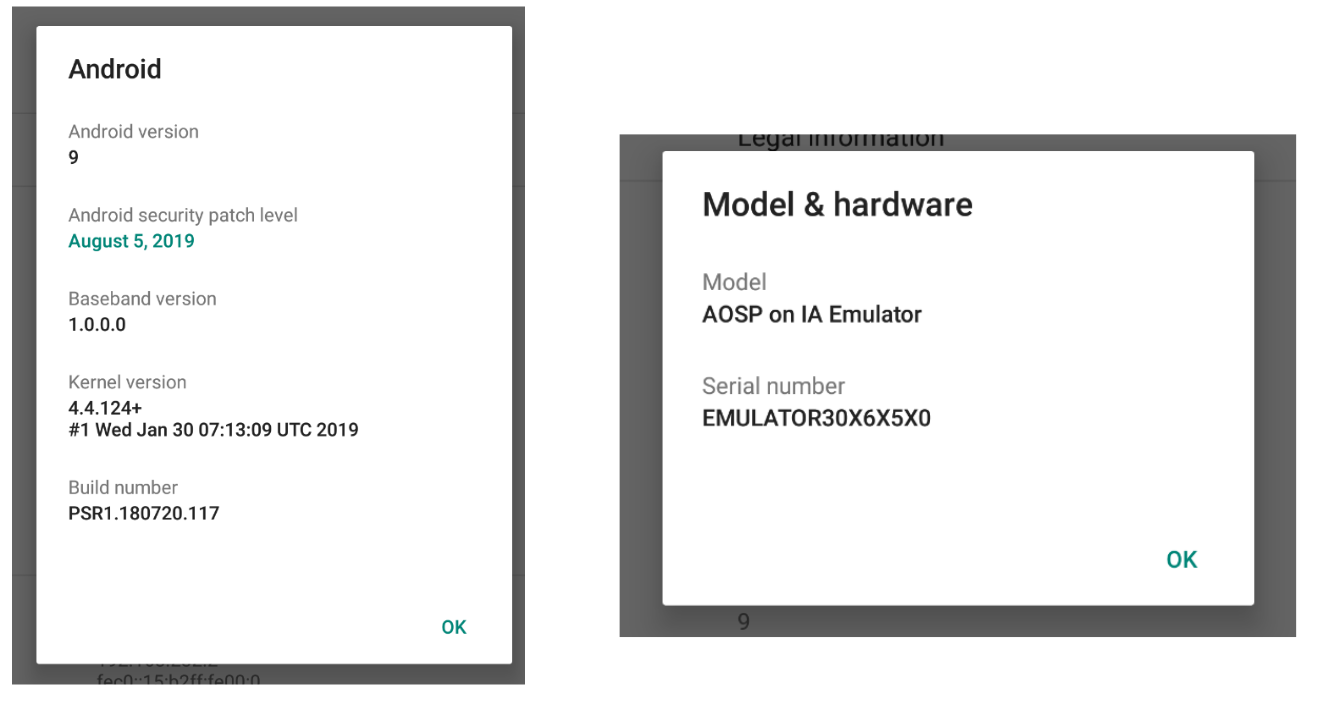
\includegraphics[scale=0.25 ]{detailemulator.png}
	\caption{Emulator Details}
\end{figure}
\pagebreak
\tocless\subsection{Details of the Compilations}
\tocless\subsubsection{Compilation 1}
\begin{itemize}
	\item Body Part: Chest
	\item Symptoms: Cough, Neusea
	\item Proposed Symptoms: Runny Nose
	\item Execution Time: 0:01:10.896734
\end{itemize}
Processor time (in \%)
\begin{figure}[H]
	\centering
	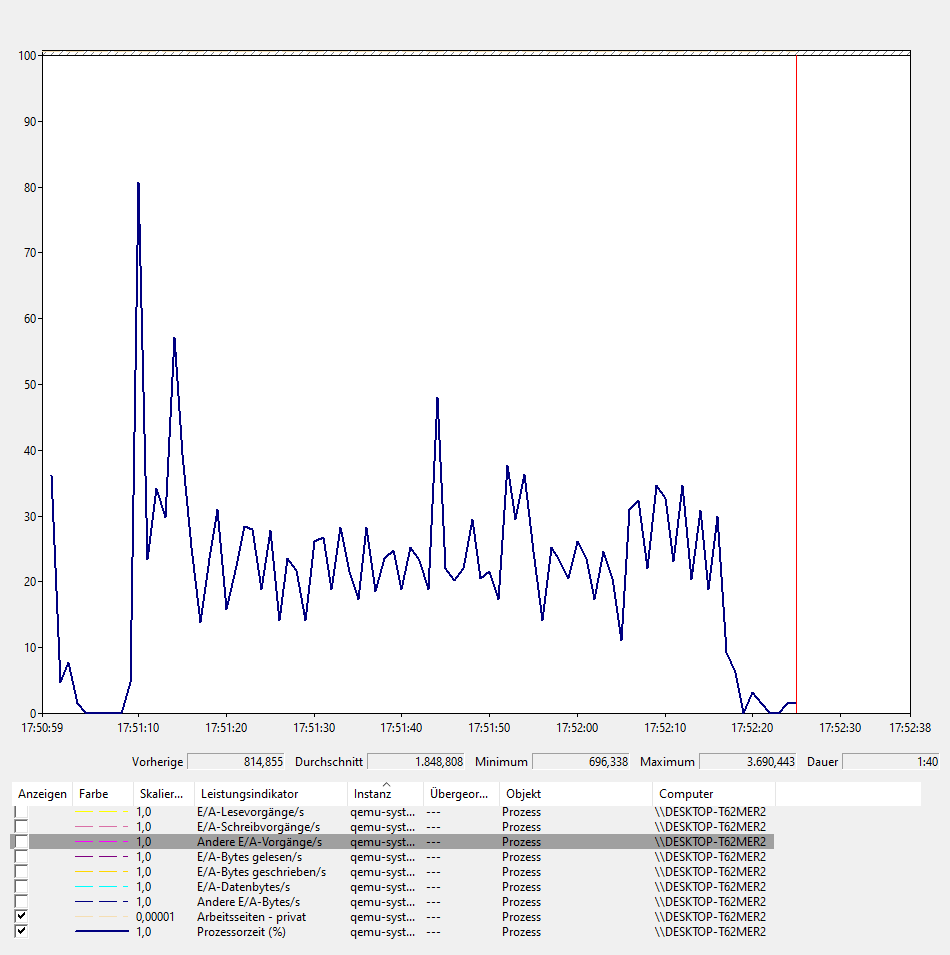
\includegraphics[scale=0.5]{COMP1.png}
	\caption{Processor Time Compilation 1}
\end{figure}

\pagebreak
\subsubsection{Compilation 2}
\begin{itemize}
	\item Body Part: Hand \& wrist 
	\item Symptoms: Joint pain(intensity: high, novality: old), Hand swelling (intensity: medium, novality: old)
	\item Proposed Symptoms: Overweight (intensity: medium, novality: new)
	\item Execution Time: 0:00:36.914100
\end{itemize}
Processor time (in \%)
\begin{figure}[H]
	\centering
	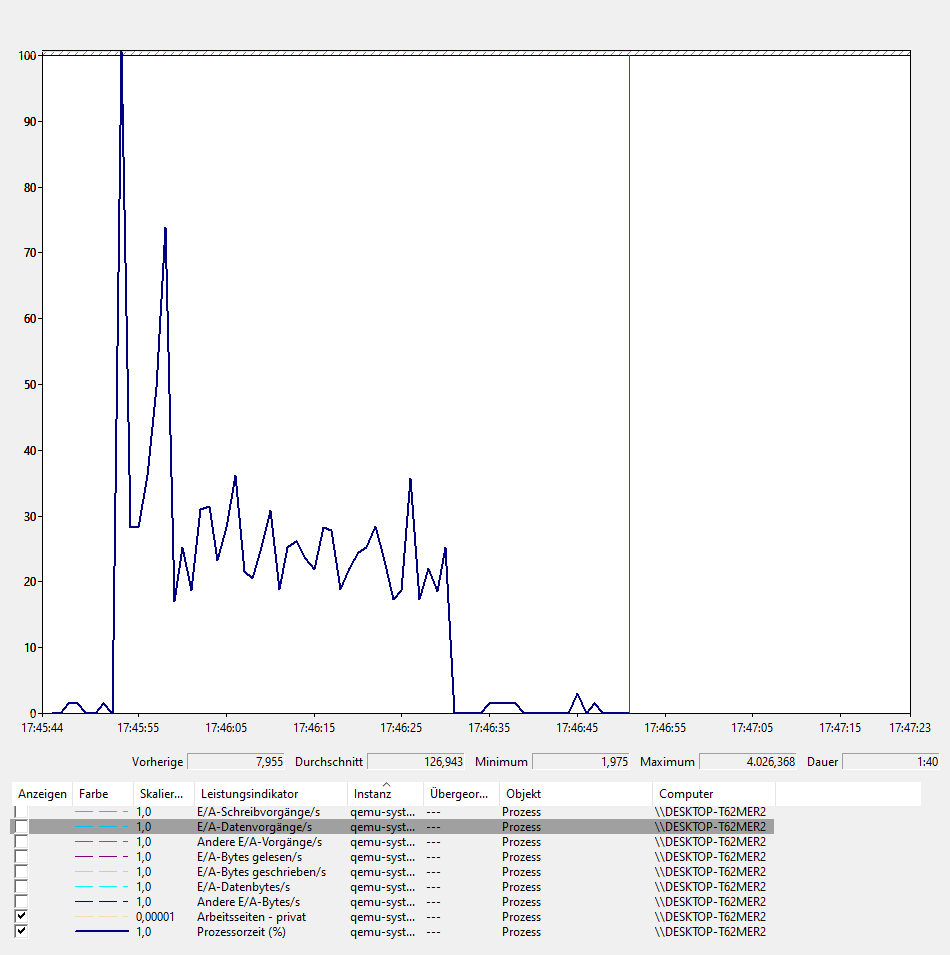
\includegraphics[scale=0.5]{COMP2.png}
	\caption{Processor Time Compilation 2}
\end{figure}

\pagebreak
\subsubsection{Compilation 3}
\begin{itemize}
	\item Body Part: Foot
	\item Symptoms: Cold feet(intensity: high, novality: old), Cramps  (intensity: medium, novality: old), Tremor at rest  (intensity: medium, novality: old)
	\item Proposed Symptoms: Tiredness (intensity: medium, novality: new)
	\item Execution Time: 0:01:15.182124
\end{itemize}
Processor time (in \%)
\begin{figure}[H]
	\centering
	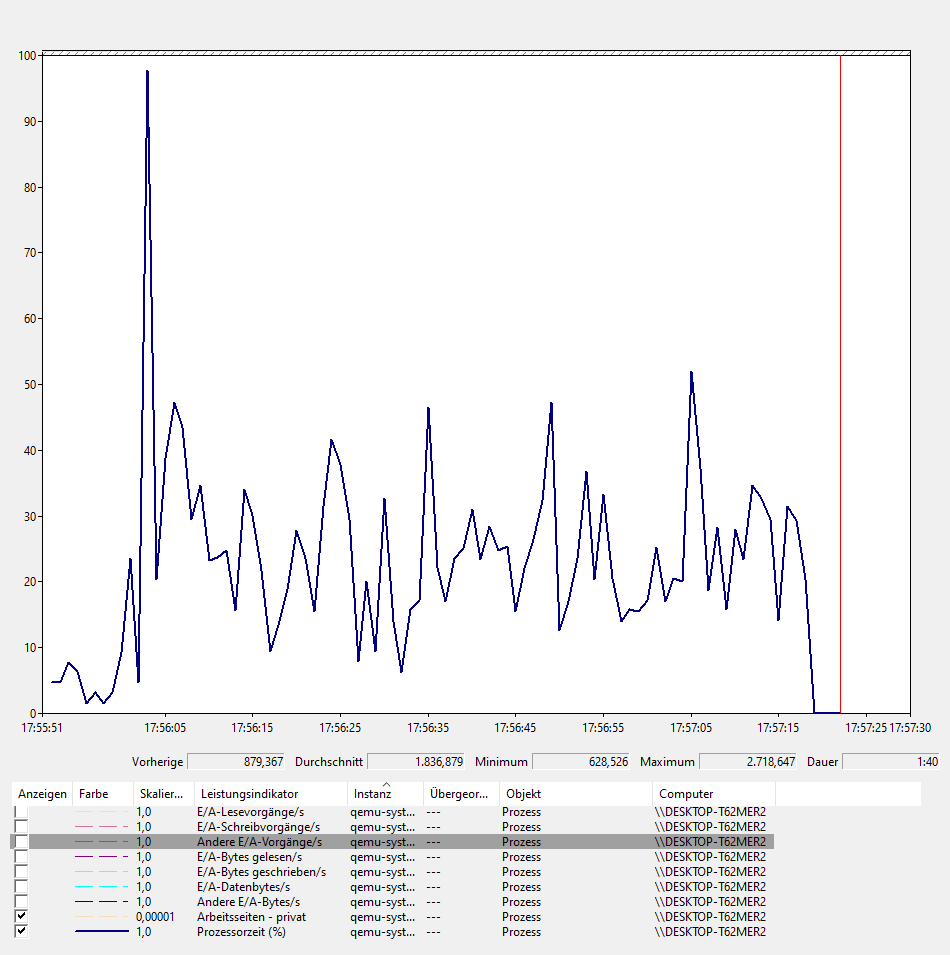
\includegraphics[scale=0.5]{COMP3.png}
	\caption{Processor Time Compilation 3}
\end{figure}

\tocless\chapter{Methods to Store Data Locally}
\tocless\section{Convert to Map}
\begin{lstlisting}[caption=Data toMap]
  static Map<String, dynamic> toMap(Diagnose pDiagnose) => {
	'id': pDiagnose.id,
	...
};
\end{lstlisting}
\tocless\section{Encode Data}
A list of diagnoses can even be saved directly. Since SharedPreference works with key-value values, these can also be easily deleted from the list by simply removing the associated key.
\begin{lstlisting}[caption=Encode Data]
  static String encode(List<Diagnose> pDiagnoses) => json.encode(
	pDiagnoses
		.map<Map<String, dynamic>>((diagnose) => Diagnose.toMap(diagnose))
		.toList(),
	);
\end{lstlisting}
\tocless\section{Decode Data}
Here the variant is displayed to directly convert a list of diagnoses.
\begin{lstlisting}[caption=Decode Data]
static List<Diagnose> decode(String pDiagnoses) =>
	(json.decode(pDiagnoses) as List<dynamic>)
	.map<Diagnose>((item) => Diagnose.fromJson(item))
.toList();
\end{lstlisting}
\tocless\section{Convert to Object (from Json)}
\begin{lstlisting}[caption=Data fromJson]
	factory Diagnose.fromJson(Map<String, dynamic> jsonData) {
		return Diagnose(
		id: jsonData['id'],
		...
		);
	}
\end{lstlisting}

\tocless\chapter{Status of the Requirements}
\begin{figure}[H]
	\centering
	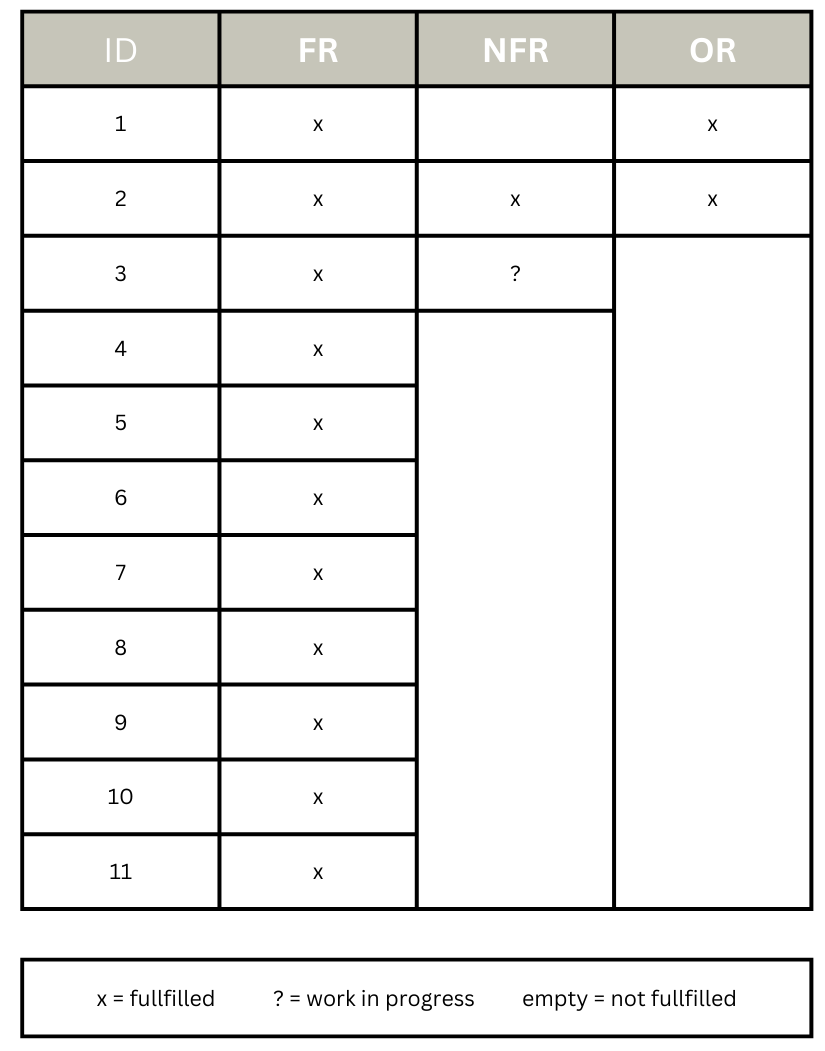
\includegraphics[scale=0.65]{frresults.png}
	\caption{Functional Requirements}
\end{figure}


\clearpage
\addcontentsline{toc}{chapter}{Literature}









